\begingroup
\tcbset{breakable/.default=false}
\chapter{力、受力分析与静力平衡}

{
\graphicspath{{/Users/dongxingxi/Documents/物理竞赛一轮资料/sample/xes-original/first-section/}}
\section{力的基本性质}
同学们可能有所耳闻，自然界中有四种基本的相互作用力，它们分别是万有引力、电磁力、
强和弱相互作用力。力（force）是物体之间相互作用的一种表现形式，当有力作用在任何一个
物体上时，它将会对力的作用产生响应，响应的形式有很多，其中最明显的就是运动状态或
形状的改变。我们将首先学习力的基本的一面，即如何对力进行测量，如何描写物质系统的
受力，在已知力作用下处于静止状态力学系统的性质。在随后的课程中将逐步深入，研究在
已知的力作用下如何预测物体未来的运动的方法，从力的宏观性质出发进入到物质世界的深处
进一步探索力的起源。


对宏观物体受力的研究是学习描写各种力最初的一步，将来可以看到，这里所学的技术对于
那些无法直观体验的对象之间相互作用的问题提供了丰富的术语和方法。为了完整描写宏观
物体所受的一个力，需要指出该力的大小、方向和作用在物体上的位置，也就是作用点，它们
合起来称为力的三要素。从更基本的观点来看，力可以用空间中的一个矢量来描写，力的三要素
一起给出了作为一个矢量的大小、方向和起点的位置。方向和作用点由传统的几何方法给出，
而力的大小则需要引入一个新的单位，为了纪念力学的奠基人，今天将力的单位取为牛顿，
用 N 来表示，将在动力学中给出其准确含义。

虽然从最基本的角度来看自然界只有四种相互作用力，而且强、弱相互作用只存在于亚原子
物理当中，也就是说宏观物体的受力全部起源于万有引力和电磁相互作用力，原则上可以根据
它们的性质以及物质的结构从微观理论出发预测出各种情况下宏观物体的受力。但是实践上以
这种方法得到宏观物体的受力实际上是不现实的，因为物质世界极大的复杂性。所以在实际的
研究过程中首先根据力的表现形式和效果对其进行分类，研究力和那些已知的、容易观察的物理量
之间的关系，最后逐步地深入探讨力的本质和起源。基于经验和观察人们发现了几种常见的力，
下面我们逐一了解一下它们。

\clearpage
\subsection{重力}

本质上讲重力是万有引力在地球表面附近的一种表现形式，它来自于地球对所有物体的吸引。
观测表明，处于地球表面附近的物体都会受到重力作用，在地球的任何地方，其方向均竖直
向下指向地面，大小正比于物体的质量，作用于物体的重心处。关于重力有几点需要说明的地方：

\begin{itemize}
  \item 将地表任何一点处物体所受重力大小 $G$ 与其质量 $m$ 的比例系数称为地表的重力
  加速度，用 $g$ 表示
  \begin{equation}
    G=mg,\qquad g\approx\SI{9.8}{\metre\per\second\squared}.
  \end{equation}

  \item 真实测量表明，地表各处的 $g$ 并不完全相同。纬度、海拔、地球形状和自转
  都会带来修正；在大多数近地竞赛题中，这些差异可以忽略。

  \item 近地问题中把重力方向定义为当地铅垂向下。它一般不严格指向地心，但在小尺度问题中
  可视为方向和大小都不变的均匀场。

  \item 在均匀重力场中，各部分所受重力的合力作用线通过质心，因而重心与质心重合。
  如果物体可以看成
  是由多个质点构成，将这些质点编号，第 $i$ 个质点的质量为 $m_i$，在固定的直角坐标系中
  的位置为 $(x_i,y_i,z_i)$ 时，质心的坐标 $(x_c,y_c,z_c)$ 为
  \begin{equation}
    x_c=\frac{\sum_i m_ix_i}{\sum_i m_i},\qquad
    y_c=\frac{\sum_i m_iy_i}{\sum_i m_i},\qquad
    z_c=\frac{\sum_i m_iz_i}{\sum_i m_i}.
  \end{equation}
\end{itemize}

\begin{origexamplebox}{}\label{ch05:ex:s01-1-1}
求一块三边长分别为 $a,b,c$ 的均匀三角板的重心位置。

\begin{center}
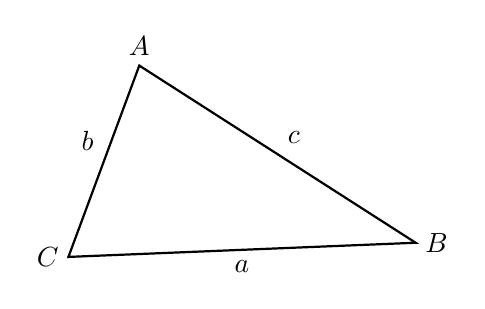
\begin{tikzpicture}[scale=0.9]
  \coordinate (A) at (0.6,2.7);
  \coordinate (B) at (4.5,0.2);
  \coordinate (C) at (-0.4,0);
  \draw[thick] (A)--node[above right] {$c$}(B)--node[below] {$a$}(C)--node[above left] {$b$}cycle;
  \node[above] at (A) {$A$};
  \node[right] at (B) {$B$};
  \node[left] at (C) {$C$};
\end{tikzpicture}
\end{center}
\end{origexamplebox}

\Needspace{6\baselineskip}\begin{xesolution}
取三角形三个顶点的位置矢量分别为 $\vec r_A,\vec r_B,\vec r_C$。先作一条中线，例如从
$A$ 连到 $BC$ 的中点 $D$。把三角板分成平行于 $BC$ 的许多极细长条，每个长条的质心都在
$AD$ 上，因而整块板的质心也在 $AD$ 上。同理，它还在其他中线上，所以质心就是三条中线的交点 $G$。

\begin{center}
\begin{tikzpicture}[scale=0.72]
  \coordinate (A) at (0.6,2.7); \coordinate (B) at (4.5,0.2); \coordinate (C) at (-0.4,0);
  \coordinate (D) at ($(B)!0.5!(C)$); \coordinate (E) at ($(C)!0.5!(A)$);
  \coordinate (F) at ($(A)!0.5!(B)$); \coordinate (G) at (barycentric cs:A=1,B=1,C=1);
  \draw[thick] (A)--(B)--(C)--cycle;
  \draw[guide] (A)--(D) (B)--(E) (C)--(F);
  \fill[Ink] (D) circle (1.3pt) node[below] {$D$};
  \fill[DeepBlue] (G) circle (2pt)
    node[above=6pt,xshift=4pt,inner sep=0pt] {$G$};
  \node[above] at (A) {$A$}; \node[right] at (B) {$B$}; \node[left] at (C) {$C$};
\end{tikzpicture}
\end{center}

中线交点将每条中线按从顶点起 $2:1$ 分割，等价地
\[
  \boxed{\vec r_G=\frac{\vec r_A+\vec r_B+\vec r_C}{3}}.
\]
边长 $a,b,c$ 只决定三角形的形状，不改变“重心为中线交点”这一结论。
\end{xesolution}

\begin{origexamplebox}{}\label{ch05:ex:s01-1-2}
求由三根均匀杆构成的三角形的重心位置，其中三杆长度分别为 $a,b,c$，满足
$a^2+b^2=c^2$。分别用 $\lambda_a,\lambda_b,\lambda_c$ 表示各杆的线密度，先求一般结果，
再讨论三杆线密度相同的情形。

\begin{center}
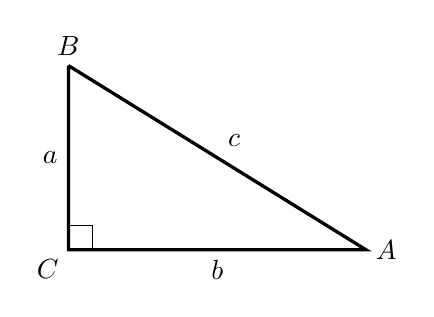
\begin{tikzpicture}[scale=0.9]
  \coordinate (C) at (0,0);
  \coordinate (B) at (0,2.6);
  \coordinate (A) at (4.2,0);
  \draw[very thick] (B)--node[left] {$a$}(C)--node[below] {$b$}(A)--node[above right] {$c$}(B);
  \draw[thin] (0,0.34)--(0.34,0.34)--(0.34,0);
  \node[above] at (B) {$B$};
  \node[below left] at (C) {$C$};
  \node[right] at (A) {$A$};
\end{tikzpicture}
\end{center}
\end{origexamplebox}

\Needspace{6\baselineskip}\begin{xesolution}
“均匀”表示每根杆内部的线密度不随位置变化，并不表示三根杆的线密度一定相等。
取直角顶点 $C$ 为原点，$CA$ 沿 $x$ 轴、$CB$ 沿 $y$ 轴。
三根杆的质量及各自中点为
\[
\begin{array}{c|c|c}
\text{杆} & \text{质量} & \text{质心坐标}\\ \hline
BC & \lambda_a a &(0,a/2)\\
CA & \lambda_b b &(b/2,0)\\
AB & \lambda_c c &(b/2,a/2)
\end{array}
\]
记总质量为 $M=\lambda_a a+\lambda_b b+\lambda_c c$。各杆的质量乘其质心坐标后相加，得到
\[
 Mx_G=\lambda_a a\cdot0+\lambda_b b\cdot\frac b2+\lambda_c c\cdot\frac b2,
\]
\[
 My_G=\lambda_a a\cdot\frac a2+\lambda_b b\cdot0+\lambda_c c\cdot\frac a2.
\]
所以一般结果为
\[
 \boxed{x_G=\frac{b(\lambda_b b+\lambda_c c)}{2M},\qquad
 y_G=\frac{a(\lambda_a a+\lambda_c c)}{2M}}.
\]
只有进一步给定 $\lambda_a=\lambda_b=\lambda_c=\lambda$，才可约去共同线密度，得到
\[
  \boxed{x_G=\frac{b(b+c)}{2(a+b+c)},\qquad
  y_G=\frac{a(a+c)}{2(a+b+c)}} ,
\]
其中 $c=\sqrt{a^2+b^2}$。这里不能套用“三角板的中线交点”：面密度均匀与线密度均匀是两个不同的质量分布。
式中分子量纲为质量乘长度、分母为质量，坐标的量纲正确。若某一杆的质量远大于另外两杆，
一般式便趋于该杆中点的坐标，也符合质心的含义。
\end{xesolution}

\begin{origexamplebox}{}\label{ch05:ex:s01-1-3}
求下面阴影的重心。

\begin{center}
\begin{tikzpicture}[scale=0.92]
  \coordinate (O) at (0.70,0);
  % Leave a visible annular gap: the sketch has R=2.20, r=0.65, l=1.20.
  \coordinate (Op) at (-0.50,0);
  \fill[TextGray!35,even odd rule] (O) circle (2.20) (Op) circle (0.65);
  \draw[thick] (O) circle (2.20);
  \draw[thick] (Op) circle (0.65);
  \fill[Ink] (O) circle (1.8pt) node[below right=2pt] {$O$};
  \fill[Ink] (Op) circle (1.8pt)
    node[below=3pt,inner sep=0pt] {$O'$};
  \draw[->,draw=Ink] (O)--++(45:2.20) node[midway,above left] {$R$};
  \draw[->,draw=Ink] (Op)--++(135:.65) node[midway,above right] {$r$};
  \draw[draw=Ink] (Op)--(O) node[pos=0.68,below=3pt] {$l$};
\end{tikzpicture}
\end{center}
\end{origexamplebox}

\Needspace{6\baselineskip}\begin{xesolution}
设薄片面密度为 $\sigma$，以大圆圆心 $O$ 为原点。把挖去的小圆看成位于 $O'$ 的“负质量”，则
\[
  M=\sigma\pi R^2,\qquad m=\sigma\pi r^2.
\]
剩余部分的质量为 $M-m$，对 $O$ 取质量矩，
\[
  (M-m)\vec r_G=M\vec 0-m\,\overrightarrow{OO'}.
\]
所以
\[
  \boxed{\vec r_G=-\frac{r^2}{R^2-r^2}\,\overrightarrow{OO'}}.
\]
\begin{center}
\begin{tikzpicture}[scale=0.62]
  \coordinate (O) at (0,0);
  \coordinate (Op) at (-0.92,0);
  \coordinate (G) at (0.42,0);
  \fill[TextGray!30,even odd rule] (O) circle (1.75) (Op) circle (0.52);
  \draw[thick] (O) circle (1.75);
  \draw[thick] (Op) circle (0.52);
  \draw[guide] (Op)--(G);
  \fill[Ink] (Op) circle (1.6pt);
  \draw[thin,TextGray] (Op)--(-1.92,0);
  \node[left=2pt,inner sep=0pt] at (-1.92,0) {$O'$};
  \fill[Ink] (O) circle (1.6pt) node[below=3pt] {$O$};
  \fill[DeepBlue] (G) circle (2pt) node[above right=2pt] {$G$};
  \draw[-{Latex[length=2.2mm]},thick,draw=DeepBlue]
    ($(O)+(0,0.34)$)--($(G)+(0,0.34)$)
    node[midway,above] {$\vec r_G$};
  \node[font=\scriptsize,text=TextGray,anchor=west] at (1.95,0.35)
    {质心在小孔的反方向};
  \draw[guide] (1.85,0.20)--(0.55,0.06);
\end{tikzpicture}\\[-0.4ex]
{\scriptsize\color{TextGray}方向示意；为便于辨认，图中 $OG$ 的长度未按比例绘制。}
\end{center}
质心位于 $OO'$ 直线上、在小孔的反方向，与 $O$ 的距离为
$lr^2/(R^2-r^2)$。这一结果要求小圆孔完全位于大圆内，即 $l+r\le R$。
\end{xesolution}

\begin{origexamplebox}{}\label{ch05:ex:s01-1-4}
已知一个质量为 $M$ 的没有盖子的圆柱形的杯子。里面开始是空的，然后往里面慢慢地注水。
进入了杯子的水和杯子的总重心会发生变化。请问重心如何变化？是否有最值？是多少？
（已知杯子底面积为 $S$，水的密度为 $\rho$，原来空杯子重心高度为 $H$，杯内允许的
最大水深为 $h_{\max}$。）
\end{origexamplebox}

\Needspace{6\baselineskip}\begin{xesolution}
设水面高度为 $h$，从杯底向上量取坐标。水的质量为 $\rho Sh$，其质心高度为 $h/2$，
因而系统质心高度为
 \begin{equation}
  z(h)=\frac{MH+\frac12\rho Sh^2}{M+\rho Sh}.
  \label{ch05:eq:cup-centre-mass}
\end{equation}
\begin{center}
\begin{tikzpicture}[scale=0.68]
  \fill[PaleBlue] (0.06,0.06) rectangle (2.64,1.45);
  \draw[very thick] (0,3.10)--(0,0)--(2.70,0)--(2.70,3.10);
  \draw[thick,draw=DeepBlue] (0.06,1.45)--(2.64,1.45);
  \draw[guide] (1.35,0)--(1.35,3.10);
  \draw[<->,draw=Ink] (-0.36,0)--(-0.36,1.45)
    node[midway,left] {$h$};
  \fill[Ink] (1.35,0.725) circle (1.7pt);
  \draw[guide] (1.45,0.725)--(3.08,0.725);
  \node[anchor=west,inner sep=0pt] at (3.12,0.725)
    {水的质心：$h/2$};
  \draw[Ink,thick] (1.27,2.48)--(1.43,2.64) (1.27,2.64)--(1.43,2.48);
  \draw[guide] (1.45,2.56)--(3.08,2.56);
  \node[anchor=west,inner sep=0pt] at (3.12,2.56)
    {空杯重心：$H$};
  \fill[DeepBlue] (1.35,1.86) circle (2pt);
  \draw[guide] (1.45,1.86)--(3.08,1.86);
  \node[anchor=west,inner sep=0pt,text=DeepBlue] at (3.12,1.86)
    {总质心：$z(h)$};
\end{tikzpicture}\\[-0.4ex]
{\scriptsize\color{TextGray}某一注水状态示意；$z(h)$ 总在 $H$ 与 $h/2$ 之间，图中具体高度不代表一般大小关系。}
\end{center}
注水时新加入的一层水位于高度 $h$，由式 \eqref{ch05:eq:cup-centre-mass} 也可直接得到
\[
  \frac{\dd z}{\dd h}=\frac{\rho S}{M+\rho Sh}\,[h-z(h)].
\]
因此，当新加水层低于当前质心时，质心下降；高于当前质心时，质心上升。极小值满足 $z(h_*)=h_*$，即
\[
  \frac12\rho S h_*^2+Mh_*-MH=0.
\]
取正根得
\[
  \boxed{h_*=z_{\min}
  =\frac{\sqrt{M^2+2M\rho SH}-M}{\rho S}}.
\]
结合题设给出的最大水深，可达的最低重心为
\[
  \boxed{z_{\min,\text{可达}}=
  \begin{cases}
    h_*, & h_{\max}\ge h_*,\\[2pt]
    \displaystyle\frac{MH+\frac12\rho S h_{\max}^2}
    {M+\rho S h_{\max}}, & h_{\max}<h_*.
  \end{cases}}
\]
第二种情形中，$0\le h\le h_{\max}$ 内有 $h<z(h)$，所以 $z(h)$ 始终随注水下降，
最小值确在装到 $h_{\max}$ 时取得。
\end{xesolution}

\begin{origexamplebox}{【思考题】}\label{ch05:ex:s01-1-5}
已知一个均匀质量的圆球壳，半径为 $R$，现在将球壳上端高度为 $h$ 的部分切下，然后
粘贴在圆球的最下面，形成一个“杯子”。求这个杯子的重心。
\end{origexamplebox}

\Needspace{6\baselineskip}\begin{xesolution}
以原球心为原点，向上为 $z$ 轴。这里的“粘贴在圆球的最下面”是指：
球冠保持原来的朝向，不作翻转，整体向下平移，使球冠顶点与原球壳最低点粘接；
球冠的圆形边缘位于最下方，构成杯子的底座。

\begin{center}
\begin{tikzpicture}[scale=0.82]
  \begin{scope}[shift={(-3.30,0)}]
    % 取示意半径 1.5、球冠高度 0.5；切口在 y=1.0。
    \draw[thick]
      (-1.12,1.00) arc[start angle=138.2,end angle=401.8,radius=1.50];
    \draw[very thick,DeepBlue]
      (-1.12,1.00) arc[start angle=138.2,end angle=41.8,radius=1.50];
    \draw[guide] (-1.12,1.00)--(1.12,1.00);
    \draw[guide] (-1.62,0)--(1.62,0);
    \draw[guide] (0,-1.65)--(0,1.75) node[above=1pt]{$z$};
    \draw[<->] (-1.72,1.50)--(-1.72,1.00) node[midway,left]{$h$};
    \fill[Ink] (0,0) circle (1.5pt) node[below right]{$O$};
    \node[DeepBlue,font=\small] at (0,-1.90) {(1) 切下上球冠};
  \end{scope}
  \draw[-{Latex[length=2.3mm]},thick,draw=TextGray] (-1.25,0.05)--(1.25,0.05);
  \node[font=\scriptsize,align=center,inner sep=0pt] at (0,0.72)
    {不翻转\\整体下移 $2R$};
  \begin{scope}[shift={(3.30,0.45)}]
    % 原球壳上方开口；灰虚线仅标出球冠原来的位置。
    \draw[thick]
      (-1.12,1.00) arc[start angle=138.2,end angle=401.8,radius=1.50];
    \draw[TextGray,dashed]
      (-1.12,1.00) arc[start angle=138.2,end angle=41.8,radius=1.50];
    \draw[guide] (-1.12,1.00)--(1.12,1.00);
    \draw[guide] (-1.62,0)--(1.62,0);
    \draw[guide] (0,-2.30)--(0,1.70) node[above=1pt]{$z$};
    % 同一球冠向下平移 2R：顶点恰好接触原球壳最低点。
    \draw[very thick,DeepBlue]
      (-1.12,-2.00) arc[start angle=138.2,end angle=41.8,radius=1.50];
    % 圆形切口的透视示意：前半实线、后半虚线。
    \draw[DeepBlue,thick]
      (-1.12,-2.00) arc[start angle=180,end angle=360,x radius=1.12,y radius=0.12];
    \draw[DeepBlue,thick,densely dashed]
      (-1.12,-2.00) arc[start angle=180,end angle=0,x radius=1.12,y radius=0.12];
    \fill[Ink] (0,0) circle (1.5pt) node[below right]{$O$};
    \fill[DeepBlue] (0,-1.50) circle (1.7pt);
    \draw[TextGray,thin] (0,-1.50)--(1.68,-1.12)--(1.92,-1.12);
    \node[font=\scriptsize,anchor=west,inner sep=0pt]
      at (1.96,-1.12) {粘接点};
    \draw[DeepBlue,thin] (1.12,-2.00)--(1.48,-2.25);
    \node[DeepBlue,font=\scriptsize,anchor=west,inner sep=0pt]
      at (1.50,-2.25) {圆形支承边缘};
    \node[DeepBlue,font=\small] at (0,-2.82) {(2) 作为底座粘贴};
  \end{scope}
\end{tikzpicture}
\\[-0.4ex]
{\scriptsize\color{TextGray}蓝色曲线表示同一球冠；右图中球冠在原球壳外部，顶点与球壳最低点相接。}
\end{center}

设球壳面密度为 $\sigma$。高为 $h$ 的薄球冠面积为 $2\pi Rh$，而对球壳水平分层有
$\dd A=2\pi R\,\dd z$，所以球冠质心高度为
\[
  z_c=\frac{\int_{R-h}^{R}z\,\dd z}{\int_{R-h}^{R}\dd z}
  =R-\frac h2.
\]
球冠原来的顶点坐标为 $R$。平移后该顶点与原球壳最低点 $-R$ 重合，
所以整个球冠向下平移了 $2R$，其质心的新坐标为
\[
  z_c'=z_c-2R=-R-\frac h2.
\]
球冠质量 $m_c=2\pi Rh\sigma$，原球壳总质量 $M_0=4\pi R^2\sigma$。
取下原位置的球冠，再把它粘到新位置，系统质量不变；相对于原球壳，质量矩的改变量为
\[
  M_0z_G=-m_cz_c+m_cz_c'
  =m_c(z_c'-z_c)=-2Rm_c.
\]
因此
\[
  z_G=\frac{-2R(2\pi Rh\sigma)}{4\pi R^2\sigma}
  =\boxed{-h}.
\]
负号表示杯子的重心在原球心下方，距原球心为 $h$。这个结果也可直接理解为：
占总质量 $h/(2R)$ 的球冠整体下降了 $2R$，所以系统质心下降 $h$。
\end{xesolution}

\subsection{弹力}

当相互接触的物体发生形变时所产生的恢复形变的力称为弹性力，胡克定律表明，当物体
形变不太大时，弹性力与形变成正比，弹簧的弹性力 $F$ 与弹簧相对于原长的形变（拉伸
或压缩）$x$ 成正比。取沿弹簧轴的有符号形变量 $x$，弹力分量与形变反向，即
\begin{equation}
  F=-kx,
\end{equation}
式中比例系数 $k$ 称为弹簧的倔强系数，也叫劲度系数，负号表示弹性力与形变反方向。
这里形变为零的位置对应弹簧原长，不一定是物体受所有外力后的平衡位置。例如竖直弹簧
悬挂物体时，平衡伸长量为 $mg/k$，该处弹力仍向上且大小为 $mg$，并不为零。
关于弹力也有几点需要注意的地方：

\begin{itemize}
  \item 当把多根弹簧并排放置共同作用时，称两弹簧并联，并联弹簧在任意位置处形变量
  相同。这里取共同连接到刚性横杆上的理想轻弹簧，讨论沿弹簧轴的小形变：共同位移为 $x$，
  第 $i$ 根弹簧提供的力为 $F_i=k_i x$，故总力为
  \[
    F=\sum_iF_i=\left(\sum_i k_i\right)x.
  \]
  与 $F=kx$ 比较，多根弹簧并联的等效劲度系数为
  \begin{equation}
    k=k_1+k_2+\cdots,
  \end{equation}
  为每根弹簧劲度系数之和。和电路类比，除了并联以外多根弹簧之间也可以串联，处于串联
  状态的弹簧在受力以后形变量并不相同；连接点质量可忽略且无其他外力时，各弹簧的张力相同。
  把各段伸长量相加，可得串联弹簧的等效劲度
  系数为
  \begin{equation}
    \frac1k=\frac1{k_1}+\frac1{k_2}+\cdots.
  \end{equation}

  \item 绳子的张力是一种弹性力，绳子和与之连接的物体之间有相互作用时，不仅绳子与
  物体之间有弹性力，而且在绳子内部也因发生相对形变而出现弹性力。这时，绳子上任一
  横截面两边互施作用力，这对作用力和反作用力称为绳子的张力，一般情况下，与绳子相应
  的比例系数 $k$ 很大，因而形变很小，可以忽略。所以绳子的张力不是由绳子的形变规律
  确定，而是由求解力学问题时确定。因而我们一般抽象出柔软不可伸长的轻绳。

  \item 物体与支撑面接触时，微观形变会产生接触力。接触力的法向分量称为支持力 $N$；
  只在光滑面模型中，合接触力才必定沿曲面法线。若表面粗糙，还要加上沿切平面的摩擦力，
  此时合接触力通常不与表面垂直。支持力和摩擦力的大小不是预先给定的，而由运动状态与约束共同决定。

  \item 所有弹力的起源均为电磁相互作用力，这一点只有从微观角度才能够发现。
\end{itemize}

\begin{origexamplebox}{}\label{ch05:ex:s01-1-6}
证明：串联弹簧的等效弹性系数小于其中任何一根弹簧的弹性系数，并解释形成这一现象的原因。
\end{origexamplebox}

\Needspace{6\baselineskip}\begin{xesolution}
两根弹簧串联时张力相同，设为 $F$。各弹簧伸长量为 $x_i=F/k_i$，总伸长量为
\[
  x=\sum_i x_i=F\sum_i\frac1{k_i}.
\]
令 $F=k_{\rm eq}x$，得
\[
  \frac1{k_{\rm eq}}=\sum_i\frac1{k_i}.
\]
因为对任意一根弹簧 $j$ 都有
\[
  \frac1{k_{\rm eq}}=\frac1{k_j}+\sum_{i\ne j}\frac1{k_i}>\frac1{k_j},
\]
所以
\[
  \boxed{k_{\rm eq}<k_j\qquad(\text{对所有 }j)}.
\]
物理上，同一个力使每根弹簧都伸长，而串联组的总伸长是各伸长量之和；与任意一根单独弹簧相比，
同力下形变更大，等效劲度自然更小。
\end{xesolution}

\subsection{滑动摩擦力、静摩擦力}

摩擦力也是一种接触力，当相互接触的物体作相对运动或有相对运动趋势时，接触面间会
产生一种阻碍相对运动或相对运动趋势的力，这种力称为摩擦力，前者称为滑动摩擦力，
后者称为静摩擦力。测量结果表明：

\begin{enumerate}[label=\arabic*.]
  \item 在库仑摩擦的近似模型中，滑动摩擦力大小与法向支持力成正比，方向与接触面上的相对滑动速度相反：
  \begin{equation}
    \vec f_k=-\mu_kN\frac{\vec v_{\rm rel}}{|\vec v_{\rm rel}|},
  \end{equation}
  其中 $\mu_k$ 称为动摩擦因数。“与表观接触面积无关”和“$\mu_k$ 为常数”都是一定条件下的理想化，
  不是对所有材料和速度都精确成立的定律。

  \item 在高中竞赛的常规库仑模型中，滑动摩擦力大小取为 $\mu_kN$，不再显式依赖速度大小。

  \item 静摩擦力是一个由平衡或共同运动条件决定的约束力，其大小满足
  \begin{equation}
    0\le |f_s|\le \mu_sN.
  \end{equation}
  只有在临界滑动时才取等号。$\mu_s$ 是最大静摩擦因数，与 $\mu_k$ 应当区分；若题目只给一个
  $\mu$，需根据所讨论的阶段明确它表示哪一个摩擦因数。
\end{enumerate}

\begin{origexamplebox}{}\label{ch05:ex:s01-1-7}
如图所示，木板 $A$ 质量为 $M$，以相对地面的速度 $v$ 在水平面上向北运动，木板上放
一质量为 $m$ 的板 $B$，各接触面间滑动摩擦因数均为 $\mu$，当木块 $B$ 也有相对地面
向东的速度 $v$ 时，试分析木块 $B$ 的受摩擦力的情况。

\begin{center}
\begin{tikzpicture}[x=1.0cm,y=1.0cm]
  \draw[fill=PaleBlue,draw=Ink,thick] (-2.5,-1.55) rectangle (2.5,1.55);
  \draw[fill=white,draw=Ink,thick] (-0.65,-0.4) rectangle (0.65,0.4);
  \node at (0,0) {$B$};
  \node[anchor=north west] at (-2.30,1.34) {$A$};
  \draw[vector] (2.9,-0.45)--(2.9,1.15) node[above] {$v$};
  \draw[vector] (-0.15,-0.72)--(1.45,-0.72) node[right] {$v$};
  \node[right] at (3.35,0.7) {北};
  \node[below] at (1.25,-1.02) {东};
\end{tikzpicture}
\end{center}
\end{origexamplebox}

\Needspace{6\baselineskip}\begin{xesolution}
取向东为 $x$ 正方向、向北为 $y$ 正方向。板 $A$ 和块 $B$ 对地速度分别为
\[
  \vec v_A=v\,\hat{\boldsymbol j},\qquad
  \vec v_B=v\,\hat{\boldsymbol i}.
\]
因而 $B$ 相对 $A$ 的滑动速度为
\[
  \vec v_{B/A}=\vec v_B-\vec v_A
  =v(\hat{\boldsymbol i}-\hat{\boldsymbol j}),
\]
方向为东南。$A$ 对 $B$ 的滑动摩擦力必须阻碍这个相对滑动，所以指向西北。

\noindent\begin{minipage}[c]{0.42\linewidth}
\centering
\begin{tikzpicture}[scale=0.64]
  \draw[axis] (-2.2,0)--(2.3,0) node[right]{东};
  \draw[axis] (0,-1.8)--(0,2.1) node[above]{北};
  \draw[vector] (0,0)--(1.4,0) node[below right]{$\vec v_B$};
  \draw[vector] (0,0)--(0,1.4) node[above left]{$\vec v_A$};
  \draw[component] (0,0)--(1.4,-1.4) node[below right]{$\vec v_{B/A}$};
  \draw[vector] (0,0)--(-1.15,1.15) node[above left]{$\vec f_{A\to B}$};
\end{tikzpicture}
\end{minipage}\hfill
\begin{minipage}[c]{0.55\linewidth}
若 $B$ 在竖直方向无加速度，则 $N=mg$，故
\[
  \boxed{\vec f_{A\to B}
  =\frac{\mu_kmg}{\sqrt2}
  (-\hat{\boldsymbol i}+\hat{\boldsymbol j})},
  \qquad |\vec f_{A\to B}|=\mu_kmg.
\]
摩擦力的方向要根据\textbf{相对速度}判断，不能只看 $B$ 的对地速度。
\end{minipage}
\end{xesolution}
}

{
\graphicspath{{/Users/dongxingxi/Documents/物理竞赛一轮资料/sample/xes-original/second-section/}}
\section{受力分析}
当一个物体受多个力作用时，需要给定所有力的大小、方向和作用点才能够完全了解它的
受力情况。对质点，多个力可合成为一个力；对刚体，若各力的作用线通过同一点，称为共点力，
也可用通过该点的合力代替。其合力为几个力的矢量和：
\begin{equation}
  \vec{F}=\sum_i\vec{F}_i.
\end{equation}
一般刚体上的非共点力还可能产生力偶；此时仅知道矢量和不足以说明转动效果，必须同时
考虑合力矩。例如两个等大反向、作用线不重合的力，合力为零，却仍能使物体转动。

当在坐标系中分析受力时，将一个给定的力向着坐标轴的方向分解对处理问题也是有帮助
的。这里采用沿正交坐标轴的投影分解；沿某个正轴的分量是有符号的数，不能把它与非负的力的大小混为一谈。

若所选单位轴为 $\hat{\boldsymbol e}$，则力沿该轴的\textbf{有符号分量}可统一写成
\[
  F_e=\vec F\cdot\hat{\boldsymbol e}=F\cos\theta.
\]
当投影方向与正轴相反时，$F_e<0$。这个负号已包含方向信息，不应再人为补一个负号。
相应的分矢量是 $F_e\hat{\boldsymbol e}$，它的大小为 $|F_e|$。若使用非正交方向作斜分解，
则需联立矢量方程，不能把每个分力都直接写成余弦投影。

\begin{origexamplebox}{}\label{ch05:ex:s02-1-8}
如图所示，有五个力 $\vec{F}_1,\vec{F}_2,\vec{F}_3,\vec{F}_4,\vec{F}_5$ 作用于一点 $O$，
构成一个正六边形的两邻边和三条对角线。设 $F_3=\SI{10}{\newton}$，试求这五个力的合力。

\begin{center}
\begin{tikzpicture}[scale=0.64]
  \coordinate (O)  at (-3,0);
  \coordinate (F1) at (-1.5,2.598);
  \coordinate (F2) at (1.5,2.598);
  \coordinate (F3) at (3,0);
  \coordinate (F4) at (1.5,-2.598);
  \coordinate (F5) at (-1.5,-2.598);

  \draw[guide,thick] (F1)--(F2)--(F3)--(F4)--(F5);
  \foreach \P in {F1,F2,F3,F4,F5}{
    \draw[-{Latex[length=2.4mm]},very thick,draw=Ink] (O)--(\P);
  }

  \node[left] at (O) {$O$};
  \node[above left] at (F1) {$F_1$};
  \node[above right] at (F2) {$F_2$};
  \node[right] at (F3) {$F_3$};
  \node[below right] at (F4) {$F_4$};
  \node[below left] at (F5) {$F_5$};
\end{tikzpicture}
\end{center}
\end{origexamplebox}

\Needspace{6\baselineskip}\begin{xesolution}
图中各力的大小就是相应矢量的几何长度。沿 $F_3$ 方向取 $x$ 轴，正六边形的边长设为 $s$，则
\[
  F_3=2s.
\]
关于 $x$ 轴对称的两对力的竖直分量相互抵消；水平分量分别为
\[
  \vec F_1+\vec F_5=s\,\hat{\boldsymbol i}
  =\frac12\vec F_3,
\]
\[
  \vec F_2+\vec F_4=3s\,\hat{\boldsymbol i}
  =\frac32\vec F_3.
\]
因而
\[
  \vec F_{\rm sum}
  =\left(\frac12+\frac32+1\right)\vec F_3
  =3\vec F_3.
\]
已知 $F_3=\SI{10}{\newton}$，所以
\[
  \boxed{F_{\rm sum}=\SI{30}{\newton}},
\]
方向与 $\vec F_3$ 相同。
\end{xesolution}

找出力学系统中每个物体受力的大小、方向和作用点的过程称为受力分析，一般来说在
静力学中主要考虑上面提到过的几种典型的受力。除了特别的假设，地面附近所有物体都受
重力，发生形变的弹性物体有弹力作用，相互接触的表面之间有可能有压力，当有压力并且
有相对运动或相对运动趋势时还可能有摩擦力。除此之外，在有的问题中还可能出现大气压
力、浮力等其它种类的力，做受力分析的时候要把所有重要的因素全部考虑方可。

虽然力的效果在物理上是一致的，但不同的力也有细微的区别。在做受力分析时，可以
将力分为两大类，一类称做主动力，例如重力、弹簧弹力等。这些力的共同特点就是它们可
由系统的状态直接确定，只要知道了物体的质量、弹簧的弹性系数和形变量以后就可以确定
其大小和方向。另一类称约束力或被动力，例如支持力、两个物体连接处的作用力等，它们
无法直接确定，是由主动力和限制物体运动约束的性质共同决定。

从建立未知量的角度看，主动力通常可由相互作用律直接写出，例如近地重力 $mg$ 和线性
弹簧力 $-kx$；约束力则通常需要与平衡方程或运动方程联立求出。这一划分是建模工具，
不是对力的微观来源进行分类。

\begin{origexamplebox}{}\label{ch05:ex:s02-1-9}
\begin{minipage}[c]{0.62\linewidth}
均匀长棒一端搁在地面上，另一端用细线系在天花板上，如图所示，若细线竖直，
试分析棒的受力情况。
\end{minipage}\hfill
\begin{minipage}[c]{0.34\linewidth}
\centering

\begin{tikzpicture}[scale=0.48]
  \draw[thick] (-3.1,-1.7)--(3.0,-1.7);
  % Model the long rod by its centre line, so its lower endpoint has
  % single-point contact with the floor rather than face contact.
  \draw[draw=Ink,line width=2.2pt,line cap=round]
    (-1.76,-1.70)--(1.67,1.69);
  \draw[thick] (1.67,1.69)--(1.67,3.05);
  \draw[thick] (0.95,3.05)--(2.39,3.05);
  \foreach \x in {1.02,1.22,...,2.32}{
    \draw[thin] (\x,3.05)--++(0.22,0.22);
  }
\end{tikzpicture}
\end{minipage}
\end{origexamplebox}

\Needspace{6\baselineskip}\begin{xesolution}
隔离木棒。对图示的非竖直木棒，需要考虑中点处的重力 $mg$、上端细线的竖直张力 $T$、
下端地面的法向力 $N$ 和水平摩擦力未知量 $f$。图中灰色虚线只表示 $f$ 的预设正方向，
并不表示摩擦力一定非零。

\begin{center}
\begin{tikzpicture}[scale=0.68]
  \coordinate (A) at (-1.8,-1.2); \coordinate (B) at (1.6,1.8); \coordinate (C) at ($(A)!0.5!(B)$);
  \draw[very thick] (A)--(B);
  \draw[vector] (B)--++(0,1.25) node[above]{$T$};
  \draw[vector] (C)--++(0,-1.35) node[below]{$mg$};
  \draw[vector] (A)--++(0,1.2) node[left]{$N$};
  \draw[-{Latex[length=2.1mm]},thick,draw=TextGray,densely dashed]
    (A)--++(1.05,0) node[pos=0.72,below=3pt,inner sep=0pt]{$f$};
  \node[below left] at (A) {$A$}; \node[right] at (B) {$B$};
\end{tikzpicture}
\end{center}

水平方向只有 $f$，由平衡条件立即得
\[
  \boxed{f=0}.
\]
力矩衡量力使物体绕参考点转动的作用，其大小为力乘参考点到作用线的垂直距离（力臂）。
取逆时针为正，平衡时各力矩的代数和为零。设木棒与水平面夹角为 $\theta$\ ($\cos\theta\ne0$)，
对下端 $A$ 取矩：$N$ 和 $f$ 的作用线都通过 $A$，力臂为零；$T$ 和 $mg$ 均竖直，
它们的力臂分别为水平距离 $L\cos\theta$ 和 $(L/2)\cos\theta$，转动趋势相反。因此
\[
  T(L\cos\theta)-mg\left(\frac L2\cos\theta\right)=0,
\]
所以
\[
  \boxed{T=\frac{mg}{2}},\qquad
  \boxed{N=mg-T=\frac{mg}{2}}.
\]
灰色虚线仅标明 $f$ 的预设正方向；求得 $f=0$ 说明接触并不意味着摩擦力非零。
若木棒恰好竖直，三个竖直力共线，力矩方程不能分别确定 $T$ 与 $N$，只能得到 $T+N=mg$。
\end{xesolution}
}

{
\graphicspath{{/Users/dongxingxi/Documents/物理竞赛一轮资料/sample/xes-original/third-section/}}
\section{质点与刚体的静力平衡}
% TikZ diagrams written for the added solutions.  They expose the forces
% and geometric quantities used in each derivation and are visually checked
% against the independently redrawn problem figures.

\tikzset{
  solbody/.style={draw=Ink,line width=0.8pt},
  solforce/.style={-{Latex[length=2.0mm]},draw=DeepBlue,line width=0.9pt},
  solgeom/.style={draw=TextGray,densely dashed,line width=0.55pt},
  soldim/.style={{Latex[length=1.4mm]}-{Latex[length=1.4mm]},draw=TextGray,line width=0.55pt},
  solpoint/.style={circle,fill=Ink,inner sep=1.2pt},
  % Labels must not carry a rectangular white mask: place them in open
  % space and use anchors/leader lines to avoid the drawing instead.
  sollabel/.style={font=\footnotesize,text=Ink,fill=none,inner sep=1pt,outer sep=1pt},
  solpanel/.style={font=\footnotesize\bfseries,text=TextGray}
}

\newcommand{\soldiagcaption}[1]{%
  \par\vspace{-0.3em}{\centering\scriptsize\color{TextGray}解图：#1\par}\vspace{0.2em}%
}

\newcommand{\soldiagOneTen}{%
\begin{center}
\begin{tikzpicture}[scale=0.88]
  \node[solpanel] at (-2.3,1.65) {(a) 铰链 $C$};
  \node[solpoint,label={[sollabel]below left:$C$}] (C) at (-2.3,0) {};
  \draw[solbody] (C) -- ++(120:1.35);
  \draw[solbody] (C) -- ++(0:1.35);
  \draw[solforce] (C) -- ++(120:1.05) node[left=5pt,sollabel] {$S$};
  \draw[solforce] (C) -- ++(0:1.10) node[above,sollabel] {$H$};
  \draw[solforce] (C) -- ++(-90:1.20) node[below,sollabel] {$mg$};
  \draw[solgeom] (C) -- ++(180:0.82);
  \draw[solgeom] ($(C)+(120:0.50)$) arc[start angle=120,end angle=180,radius=0.50];
  \node[sollabel] at (-3.03,0.30) {$60^\circ$};

  \node[solpanel] at (2.15,1.65) {(b) 铰链 $D$};
  \node[solpoint,label={[sollabel]below left=4pt:$D$}] (D) at (2.15,0) {};
  \draw[solbody] (D) -- ++(60:1.45)
    node[pos=.68,right=4pt,sollabel] {$DB$};
  \draw[solbody] (D) -- ++(180:1.25);
  \draw[solforce] (D) -- ++(180:1.10) node[above,sollabel] {$H$};
  \draw[solforce] (D) -- ++(-30:1.15) node[right,sollabel] {$F_{\min}$};
  \draw[solgeom] (D) -- ++(150:1.05);
  \draw[solgeom] ($(D)+(0.35,0.61)$) -- ++(-30:0.22) -- ++(-120:0.22);
\end{tikzpicture}
\soldiagcaption{先由 $C$ 点平衡求出杆 $CD$ 的轴力，再在 $D$ 点取垂直于 $DB$ 的分量。}
\end{center}}

\newcommand{\soldiagOneEleven}{%
\begin{center}
\begin{tikzpicture}[scale=1]
  \node[solpanel] at (-2.3,2.2) {(a) 小球受力};
  \coordinate (O) at (-2.3,0);
  \draw[solbody] (O) circle (.42);
  \draw[solforce] (O)--++(102:1.65) node[above left,sollabel] {$N_1$};
  \draw[solforce] (O)--++(-18:1.65) node[right,sollabel] {$N$};
  \draw[solforce] (O)--++(-90:1.60) node[below,sollabel] {$mg$};
  \node[solpanel] at (2.35,2.2) {(b) 沿下斜面投影};
  \draw[solgeom,->] (.55,.8)--(4.15,.8) node[right,sollabel] {向上};
  \draw[solforce] (1.1,.20)--(3.8,.20) node[midway,above=4pt,sollabel] {$N\sin\theta$};
  \draw[solforce] (3.8,-.65)--(1.1,-.65) node[midway,below=4pt,sollabel] {$mg\sin\alpha$};
  \node[sollabel] at (2.4,-1.55) {$N_1$ 的投影为零};
\end{tikzpicture}
\soldiagcaption{$N_1$ 垂直于下斜面，故沿下斜面只需平衡 $N$ 和 $mg$ 的分量。}
\end{center}}

\newcommand{\soldiagOneTwelve}{%
\begin{center}
\begin{tikzpicture}[scale=1]
  \coordinate (O) at (0,0);
  \draw[solbody] (O) circle (.35);
  \draw[solgeom] (0,-2.25)--(0,2.25);
  \draw[solgeom,->] (-1.55,0)--(2.45,0) node[right,sollabel] {$x$};
  \draw[solforce] (O)--++(103:2.10) node[above left,sollabel] {$N_1$};
  \draw[solforce] (O)--++(-38:2.10) node[below right,sollabel] {$N_2$};
  \draw[solforce] (O)--++(-90:2.00) node[below left,sollabel] {$mg$};
  \draw[solgeom] (90:1.25) arc[start angle=90,end angle=103,radius=1.25];
  \draw[TextGray,thin] (96.5:1.25)--(-1.05,1.35);
  \node[left,sollabel] at (-1.05,1.35) {$\theta_1$};
  \draw[solgeom] (-90:.95) arc[start angle=-90,end angle=-38,radius=.95];
  \draw[TextGray,thin] (-64:.95)--(1.55,-.58);
  \node[right,sollabel] at (1.55,-.58) {$\theta_2$};
\end{tikzpicture}
\soldiagcaption{$N_1$ 与竖直向上的夹角为 $\theta_1$；$N_2$ 与竖直向下的夹角为 $\theta_2$，因为支持力分别垂直于对应斜面。}
\end{center}}

\newcommand{\soldiagOneThirteen}{%
\begin{center}
\begin{tikzpicture}[scale=0.82]
  \node[solpanel] at (-2.45,2.15) {(a) 接触几何};
  \coordinate (O) at (-2.45,1.55);
  \coordinate (A) at (-3.25,-0.85);
  \coordinate (C) at (-2.45,0.05);
  \fill[Ink] (O) circle (1.4pt) node[above,sollabel] {$O$};
  \fill[Ink] (A) circle (1.4pt) node[below left,sollabel] {$A$};
  \fill[Ink] (C) circle (1.4pt) node[right,sollabel] {$C$};
  \draw[solbody] (O)--(A) node[midway,left,sollabel] {$d_0$};
  \draw[solbody] (A)--(C);
  \draw[TextGray,thin] ($(A)!.5!(C)$)--(-1.85,-.12);
  \node[right,sollabel] at (-1.85,-.12) {$R+r$};
  \draw[solgeom] (A)--(-1.55,-0.85);
  \draw[solgeom] (O)--(-2.45,-1.10);
  \draw[solgeom] ($(O)+(0,-0.55)$) arc[start angle=-90,end angle=-108.5,radius=0.55];
  \draw[TextGray,thin] ($(O)+(-99.25:.55)$)--(-3.15,1.04);
  \node[left,sollabel] at (-3.15,1.04) {$\theta$};
  \draw[solgeom] ($(A)+(0.55,0)$) arc[start angle=0,end angle=48,radius=0.55];
  \node[sollabel] at (-2.57,-0.56) {$\beta$};

  \node[solpanel] at (2.15,2.15) {(b) 大球 $A$ 受力};
  \node[solpoint,label={[sollabel]right=4pt:$A$}] (P) at (2.15,0) {};
  \draw[solforce] (P)--++(71.5:1.45) node[above,sollabel] {$T$};
  \draw[solforce] (P)--++(-132:1.18) node[below left,sollabel] {$N$};
  \draw[solforce] (P)--++(180:1.05) node[above left,sollabel] {$Q$};
  \draw[solforce] (P)--++(-90:1.30) node[below,sollabel] {$Mg$};
  \draw[solgeom] (P)--++(180:1.25);
  \draw[solgeom] ($(P)+(180:0.54)$)
    arc[start angle=180,end angle=228,radius=0.54];
  \node[sollabel] at ($(P)+(204:0.78)$) {$\beta$};
\end{tikzpicture}
\soldiagcaption{$\beta$ 由三球接触几何确定；两大球刚分离时令接触力 $Q=0$。}
\end{center}}

\newcommand{\soldiagOneFourteen}{%
\begin{center}
\begin{tikzpicture}[scale=0.92]
  \node[solpanel] at (-2.4,2.05) {(a) 切线几何};
  \coordinate (O) at (-2.40,1.55);
  \coordinate (C) at (-3.05,-0.55);
  % P is the tangent point for R=.96; hence CP is perpendicular to OP.
  \coordinate (P) at (-2.101,-0.405);
  \draw[solbody] (C) circle (0.96);
  \fill[Ink] (O) circle (1.4pt) node[above,sollabel] {$O$};
  \fill[Ink] (C) circle (1.4pt) node[below left,sollabel] {$C$};
  \fill[Ink] (P) circle (1.2pt) node[right,sollabel] {$P$};
  \draw[solbody] (O)--(C);
  \node[sollabel] at (-3.30,.08) {$l$};
  \draw[solbody] (O)--(P);
  \draw[solbody] (C)--(P) node[pos=.42,below=5pt,sollabel] {$R$};
  \draw[solgeom] (O)--++(0,-2.45);
  \draw[solgeom] ($(P)+(171.3:.16)$)--++(81.3:.16)--++(-8.7:.16);
  \draw[draw=TextGray] ($(O)+(-107.2:.60)$) arc[start angle=-107.2,end angle=-90,radius=.60];
  \draw[draw=TextGray] ($(O)+(-90:.80)$) arc[start angle=-90,end angle=-81.3,radius=.80];
  \draw[draw=TextGray] ($(O)+(-107.2:1.10)$) arc[start angle=-107.2,end angle=-81.3,radius=1.10];
  \node[sollabel] at (-2.90,.82) {$\theta$};
  \node[sollabel] at (-1.92,.79) {$\psi$};
  \draw[TextGray,thin] ($(O)+(-94.25:1.10)$)--(-3.85,.40);
  \node[left,sollabel] at (-3.85,.40) {$\delta$};

  \node[solpanel] at (2.05,2.05) {(b) 球的合力图};
  \node[solpoint] (G) at (2.05,0) {};
  \draw[solforce] ($(G)+(-.04,0)$)--++(72.8:1.35) node[above right,sollabel] {$S$};
  % At P the upper-rope tension points from P to O, i.e. along the
  % tangent, almost vertically upward in panel (a).
  \draw[solforce] ($(G)+(.04,0)$)--++(98.7:1.13) node[above left,sollabel] {$T$};
  \draw[solforce] (G)--++(-90:1.22) node[below,sollabel] {$m_1g$};
  \draw[solforce] ($(G)+(.18,-.04)$)--++(-90:.82) node[right=3pt,sollabel] {$T$};
  \draw[solgeom] (G)--++(0,1.25);
\end{tikzpicture}
\soldiagcaption{$\delta=\theta+\psi$ 且 $\sin\delta=R/l$；绕绳对球的作用等于两端张力的矢量和。}
\end{center}}

\newcommand{\soldiagOneFifteen}{%
\begin{center}
\begin{tikzpicture}[scale=0.78]
  \draw[solbody] (-2,-1.55)--(-2,2.00);
  \draw[solbody] (2,2.00)--(2,-1.55);
  \draw[solbody] (-2.35,-1.55)--(2.35,-1.55);
  \coordinate (A) at (-0.90,-0.45);
  \coordinate (B) at (0.90,0.815);
  \draw[solbody] (A) circle (1.10);
  \draw[solbody] (B) circle (1.10);
  \draw[solgeom] (A)--(B);
  \draw[solgeom] (A)--++(2.00,0);
  \draw[solgeom] ($(A)+(0:.55)$) arc[start angle=0,end angle=35.1,radius=.55];
  \node[sollabel] at ($(A)+(17.6:.78)$) {$\beta$};
  \draw[solforce] (-2,-0.45)--++(-0.95,0) node[left,sollabel] {$N_2$};
  \draw[solforce] (2,0.815)--++(0.95,0) node[right,sollabel] {$N_2$};
  \draw[soldim] (2.48,-0.45)--(2.48,0.815);
  \node[sollabel,right] at (2.48,0) {$2r\sin\beta$};
  \draw[solforce] (0,-0.25)--(0,-2.02) node[below,sollabel] {$Mg$};
  \draw[TextGray,thin] (2,-1.55)--(2.72,-1.72);
  \node[right,sollabel] at (2.72,-1.72) {倾覆边缘};
\end{tikzpicture}
\soldiagcaption{两侧壁受到一对等大反向水平力，形成力偶 $N_2(2r\sin\beta)$。}
\end{center}}

\newcommand{\soldiagOneSixteen}{%
\begin{center}
\begin{tikzpicture}[scale=0.72]
  \coordinate (A) at (-3,-1.35);
  \pgfmathsetmacro{\sone}{.52*(1+sin(25))/cos(25)}
  \draw[solbody] (-3,-1.65)--(-3,2.05);
  \draw[solbody] (A)--++(25:6.90);
  \foreach \i/\lab in {0/1,1/2,2/3}{
    \coordinate (P\lab) at ($(A)+(25:{\sone+1.04*\i})$);
    \coordinate (C\lab) at ($(P\lab)+(115:0.52)$);
    \draw[solbody] (C\lab) circle (0.52);
    \draw[solforce] (P\lab)--++(115:0.92);
    \ifnum\lab=1
      \draw[TextGray,thin] ($(P\lab)+(115:.92)$)--(-3.30,.40);
      \node[left,sollabel] at (-3.30,.40) {$N_1$};
    \else
      \node[above left,sollabel] at ($(P\lab)+(115:.92)$) {$N_{\lab}$};
    \fi
  }
  \fill[Ink] (A) circle (1.2pt) node[below left,sollabel] {$A$};
  \draw[soldim] ($(A)+(25:0.05)+(115:-0.32)$)--($(A)+(25:\sone)+(115:-0.32)$);
  \node[sollabel] at (-2.54,-1.82) {$s_1$};
  \draw[solgeom] ($(A)+(25:.30)$) arc[start angle=25,end angle=90,radius=.30];
  \draw[TextGray,thin] ($(A)+(57.5:.30)$)--(-3.58,-1.06);
  \node[left,sollabel] at (-3.58,-1.06) {$\theta$};
  \node[sollabel] at (0.55,-0.65) {$s_2=s_1+2r$};
  \node[sollabel] at (2.05,-0.05) {$s_3=s_1+4r$};
\end{tikzpicture}
\soldiagcaption{接触点沿板的位置为 $s_1,s_2,s_3$，板对各圆柱的支持力均垂直于板。}
\end{center}}

\newcommand{\soldiagOneSeventeen}{%
\begin{center}
\begin{tikzpicture}[scale=0.82]
  \coordinate (A) at (-0.40,-1.25);
  \coordinate (B) at ($(A)+(60:3.15)$);
  \draw[solbody,line width=1.2pt] (A)--(B);
  \draw[solbody] (-2.75,-1.25)--(2.55,-1.25);
  \draw[solbody] (B).. controls ($(B)+(210:1.10)$) and (-1.15,0.63)..(-2.55,0.55);
  \draw[solgeom] (B)--++(180:1.75);
  \draw[solgeom] ($(A)+(0.72,0)$) arc[start angle=0,end angle=60,radius=0.72];
  \node[sollabel] at (0.50,-0.88) {$\beta$};
  \draw[solgeom] ($(B)+(-0.68,0)$) arc[start angle=180,end angle=210,radius=0.68];
  \draw[TextGray,thin] ($(B)+(195:.68)$)--(-.40,1.82);
  \node[above left,sollabel] at (-.40,1.82) {$\gamma$};
  \draw[solgeom] ($(B)+(210:0.82)$) arc[start angle=210,end angle=240,radius=0.82];
  \draw[TextGray,thin] ($(B)+(225:.82)$)--(1.35,.95);
  \node[right,sollabel] at (1.35,.95) {$30^\circ$};
  \draw[solforce] (B)--++(210:1.45) node[below left=3pt,sollabel] {$T$};
  \coordinate (G) at ($(A)!0.5!(B)$);
  \draw[solforce] (G)--++(-90:0.76)
    node[pos=0.62,right=4pt,sollabel] {$4mg$};
  \fill[Ink] (A) circle (1.3pt) node[below,sollabel] {铰链};
  \node[sollabel] at (-1.82,0.90) {钢索切线};
\end{tikzpicture}
\soldiagcaption{一侧斜壁重为 $4mg$；斜壁的力矩平衡与屋面整体的竖直平衡必须同时满足。}
\end{center}}

\newcommand{\soldiagOneEighteen}{%
\begin{center}
\begin{tikzpicture}[scale=0.88]
  \draw[solbody] (-2.65,-0.85)--(2.75,-0.85);
  \draw[solbody,fill=white] (-1.00,-0.85) rectangle (1.00,0.55);
  \coordinate (G) at (0,-0.15);
  \draw[solforce] (1.00,0.12)--++(30:1.55) node[above right,sollabel] {$F$};
  \draw[solforce] (G)--++(90:1.35) node[above,sollabel] {$N$};
  \draw[solforce] (G)--++(-90:1.35) node[below,sollabel] {$Mg$};
  \draw[solforce] (-0.80,-0.85)--++(180:1.25)
    node[above left=2pt,sollabel] {$f=\mu N$};
  \draw[solgeom] (1.00,0.12)--++(0:1.25);
  \draw[solgeom] ($(1.00,0.12)+(0:0.68)$) arc[start angle=0,end angle=30,radius=0.68];
  \node[sollabel] at (1.82,0.33) {$\alpha$};
  \draw[solgeom,-{Latex[length=1.5mm]}] (1.55,-1.15)--(2.55,-1.15)
    node[midway,below,sollabel] {匀速};
\end{tikzpicture}
\soldiagcaption{沿运动方向有 $F\cos\alpha=f$；拉力的竖直分量使支持力减为 $N=Mg-F\sin\alpha$。}
\end{center}}

\newcommand{\soldiagOneNineteen}{%
\begin{center}
\begin{tikzpicture}[scale=0.82]
  \node[solpanel] at (-2.20,1.70) {(a) 两接触点};
  \coordinate (O) at (-3.55,0);
  \draw[solbody] (O)--(-0.55,1.15);
  \draw[solbody] (O)--(-0.55,-1.15);
  \draw[solbody] (-1.55,0) circle (0.72);
  \coordinate (U) at (-1.808,0.672); \coordinate (L) at (-1.808,-0.672);
  \draw[solforce] (U)--++(-69:0.92);
  \draw[solforce] (U)--++(201:0.88);
  \draw[solforce] (L)--++(69:0.92);
  \draw[solforce] (L)--++(159:0.88);
  \node[sollabel] at (-1.25,.22) {$N$};
  \node[sollabel] at (-1.25,-.22) {$N$};
  \node[sollabel] at (-2.67,.63) {$\mu N$};
  \node[sollabel] at (-2.67,-.63) {$\mu N$};
  \draw[solgeom] (O)--(-0.65,0);
  \draw[solgeom] ($(O)+(0.78,0)$) arc[start angle=0,end angle=21,radius=0.78];
  \draw[TextGray,thin] ($(O)+(10.5:.78)$)--(-3.53,-.72);
  \node[left,sollabel] at (-3.53,-.72) {$\theta/2$};

  \node[solpanel] at (2.55,1.70) {(b) 沿角平分线的合力};
  \draw[solgeom] (0.70,0)--(4.45,0);
  \fill[Ink] (2.55,0) circle (1.2pt);
  \draw[solforce] (2.55,0.30)--++(0:1.55)
    node[right,sollabel] {$2N\sin(\theta/2)$};
  \draw[solforce] (2.55,-0.30)--++(180:1.55);
  \node[sollabel,below=3pt] at (1.78,-.30) {$2\mu N\cos(\theta/2)$};
  \node[sollabel] at (3.45,0.70) {向外};
  \node[sollabel] at (1.65,-1.20) {向内};
\end{tikzpicture}
\soldiagcaption{正压力的合力向外，极限摩擦力的合力沿角平分线指向 $O$。}
\end{center}}

\newcommand{\soldiagOneTwenty}{%
\begin{center}
\begin{tikzpicture}[scale=0.82]
  \coordinate (A) at (-2.7,0);
  \coordinate (B) at (2.7,0);
  \draw[solbody] (-2.7,-1.1)--(-2.7,2.0);
  \draw[solbody,line width=1.15pt] (A)--(B);
  \draw[solbody] (B)--(-2.7,1.65);
  \fill[Ink] (A) circle (1.2pt) node[below left,sollabel] {$A$};
  \fill[Ink] (B) circle (1.2pt) node[below right,sollabel] {$B$};
  \coordinate (P) at (-0.90,0);
  \fill[Ink] (P) circle (1.2pt) node[above=4pt,sollabel] {$P$};
  \draw[solforce] (A)--++(0:1.05) node[below,sollabel] {$N$};
  \draw[solforce] (A)--++(90:1.10) node[left,sollabel] {$f$};
  \draw[solforce] (B)--++(163:1.32) node[above,sollabel] {$T$};
  \draw[solforce] (0,0)--++(-90:1.05) node[below,sollabel] {$Mg$};
  \draw[solforce] (P)--++(-90:1.05) node[below,sollabel] {$mg$};
  \draw[solgeom] ($(B)+(-0.72,0)$) arc[start angle=180,end angle=163,radius=0.72];
  \draw[TextGray,thin] ($(B)+(171.5:.72)$)--(2.05,-.40);
  \node[right,sollabel] at (2.05,-.40) {$\theta$};
  \draw[soldim] ($(A)+(0,-0.58)$)--($(P)+(0,-0.58)$);
  \node[sollabel] at (-1.46,-0.78) {$y$};
\end{tikzpicture}
\soldiagcaption{附加重物放在距 $A$ 为 $y$ 处；对 $A$ 取矩可直接消去 $N$、$f$。}
\end{center}}

\newcommand{\soldiagOneTwentyOne}{%
\begin{center}
\begin{tikzpicture}[scale=0.86]
  \coordinate (A) at (-2.2,-0.85);
  \coordinate (B) at (2.05,0.95);
  \draw[solbody] (-2.75,-0.85)--(2.75,-0.85);
  \draw[solbody,line width=1.2pt] (A)--(B);
  \draw[solforce] (B)--++(113:1.25) node[above,sollabel] {$F\perp$ 杆};
  \coordinate (G) at ($(A)!0.5!(B)$);
  \draw[solforce] (G)--++(-90:1.18) node[below,sollabel] {$mg$};
  \draw[solforce] (A)--++(90:1.18) node[left,sollabel] {$N$};
  \draw[solforce] (A)--++(0:1.08) node[below,sollabel] {$f$};
  \draw[solgeom] ($(A)+(0.72,0)$) arc[start angle=0,end angle=23,radius=0.72];
  \draw[TextGray,thin] ($(A)+(11.5:.72)$)--(-.70,-.42);
  \node[right,sollabel] at (-.70,-.42) {$\theta$};
\end{tikzpicture}
\soldiagcaption{外力始终与杆垂直；地板处的 $f/N$ 随抬起角度变化。}
\end{center}}

\newcommand{\soldiagOneTwentyTwo}{%
\begin{center}
\begin{tikzpicture}[scale=0.82]
  \node[solpanel] at (-2.15,1.95) {(a) 中间结点};
  \node[solpoint] (C) at (-2.15,0) {};
  \draw[solforce] (C)--++(145:1.25) node[above left,sollabel] {$T$};
  \draw[solforce] (C)--++(35:1.25) node[above right,sollabel] {$T$};
  \draw[solforce] (C)--++(-90:1.30) node[below,sollabel] {$Mg$};
  \draw[solgeom] (C)--++(1.45,0);
  \node[sollabel] at (-1.45,0.25) {$\beta$};

  \node[solpanel] at (2.15,1.95) {(b) 圆环 $A$};
  \draw[solbody] (0.70,0.72)--(3.65,0.72);
  \draw[solbody] (2.15,0.72) circle (0.20);
  \draw[solforce] (2.15,0.62)--++(-35:1.25) node[below right,sollabel] {$T$};
  \draw[solforce] (2.15,0.92)--++(90:0.82) node[midway,right,sollabel] {$N$};
  \draw[solforce] (2.15,0.52)--++(-90:1.02) node[below,sollabel] {$mg$};
  \draw[solforce] (2.15,0.76)--++(180:1.00)
    node[above left=2pt,sollabel] {$f$};
\end{tikzpicture}
\soldiagcaption{结点给出 $2T\sin\beta=Mg$；圆环的支持力还要承担细线的竖直分量。}
\end{center}}

\newcommand{\soldiagOneTwentyThree}{%
\begin{center}
\begin{tikzpicture}[scale=0.82]
  \node[solpanel,align=center] at (-3.00,2.35) {(a) 绳圈在圆锥\\上的位置};
  \coordinate (A) at (-3.00,1.60);
  \pgfmathsetmacro{\solConeHalfAngle}{atan(1.55/2.95)}
  \pgfmathsetmacro{\solConeRingRadius}{1.78*1.55/2.95}
  \draw[solbody,line width=1.05pt] (-4.55,-1.35)--(A)--(-1.45,-1.35);
  \draw[solgeom] (A)--(-3.00,-1.55) node[below,sollabel] {轴};
  \draw[solbody,line width=1.05pt] ({-3-\solConeRingRadius},-.18)
    arc[start angle=180,end angle=360,x radius=\solConeRingRadius,y radius=.20];
  \draw[solgeom] ({-3-\solConeRingRadius},-.18)
    arc[start angle=180,end angle=0,x radius=\solConeRingRadius,y radius=.20];
  \draw[solgeom] (-3.00,-0.18)--({-3+\solConeRingRadius},-.18)
    node[midway,above,sollabel] {$\rho$};
  \draw[<->,draw=TextGray] (-4.28,-.18)--(-4.28,1.60)
    node[midway,left,sollabel] {$z=\rho\cot\delta$};
  \draw[draw=TextGray] ($(A)+(-90:.66)$)
    arc[start angle=-90,end angle={-90+\solConeHalfAngle},radius=.66];
  \draw[TextGray,thin] ($(A)+({-90+\solConeHalfAngle/2}:.66)$)--(-1.65,1.43);
  \node[right,sollabel] at (-1.65,1.43) {$\delta=\alpha/2$};

  \node[solpanel,align=center] at (2.10,2.35) {(b) 纬圈微元\\径向--竖直截面};
  \coordinate (P) at (2.10,-.20);
  \draw[solgeom] (P)--($(P)+(2.05,0)$) node[right,sollabel] {水平径向};
  \draw[solgeom] ($(P)+(0,-1.65)$)--($(P)+(0,1.65)$);
  \node[sollabel,right=4pt] at ($(P)+(0,1.55)$) {竖直};
  % Numerical parameters never redefine a mathematical symbol such as delta.
  \draw[solbody,line width=1.05pt]
    ($(P)+({90+\solConeHalfAngle}:1.55)$)--($(P)+({-90+\solConeHalfAngle}:1.55)$);
  \fill[Ink] (P) circle (1.3pt);
  \draw[solforce] (P)--++(180:1.28) node[left,sollabel] {$T\,\mathrm d\varphi$};
  \draw[solforce] (P)--++(\solConeHalfAngle:1.55) node[above right,sollabel] {$\mathrm dN$};
  \draw[solforce] (P)--++(-90:1.20) node[below,sollabel] {$\mathrm dm\,g$};
  \draw[solgeom] ($(P)+(0:.78)$) arc[start angle=0,end angle=\solConeHalfAngle,radius=.78];
  \node[sollabel] at ($(P)+({\solConeHalfAngle/2}:1.03)$) {$\delta$};
\end{tikzpicture}
\soldiagcaption{左图先标出水平纬圈；右图把该圈微元放入径向--竖直截面，张力合力水平向内，支持力向外且向上。}
\end{center}}

\newcommand{\soldiagOneTwentyFour}{%
\begin{center}
\begin{tikzpicture}[scale=0.86]
  \coordinate (O) at (0,0);
  \draw[solbody] (O) ++(0:1.65) arc[start angle=0,end angle=90,radius=1.65];
  \draw[solbody] (-0.15,-0.08)--(1.82,-0.08);
  \fill[Ink] (O) circle (1.2pt) node[below left,sollabel] {$O$};
  \coordinate (P) at ($(O)+(48:1.65)$);
  \fill[Ink] (P) circle (1.2pt);
  \draw[solgeom] (O)--(P) node[midway,above left=5pt,sollabel] {$R$};
  \draw[solgeom] (O)--++(0:1.15);
  \draw[solgeom] ($(O)+(0:0.62)$) arc[start angle=0,end angle=48,radius=0.62];
  \node[sollabel] at (0.85,0.20) {$\varphi$};
  \draw[solforce] (P)--++(138:1.20) node[above left,sollabel] {$T+\mathrm dT$};
  \draw[solforce] (P)--++(-42:1.08) node[below right,sollabel] {$T$};
  \draw[solforce] (P)--++(48:0.95) node[above right,sollabel] {$\mathrm dN$};
  \draw[solforce] (P)--++(-90:1.15);
  % 重力标记单列在图下方，避免同时压住竖直力箭头和斜向张力箭头。
  \node[sollabel] at (1.08,-0.42) {$\lambda gR\,\mathrm d\varphi$};
  \node[sollabel] at (-1.60,0.95) {$\mathrm ds=R\,\mathrm d\varphi$};
\end{tikzpicture}
\soldiagcaption{微元两端张力之差平衡重力的切向分量；沿 $\varphi$ 增大方向张力增加。}
\end{center}}

\newcommand{\soldiagOneTwentyFive}{%
\begin{center}
\begin{tikzpicture}[scale=0.80]
  \draw[solbody] (0,0.45) circle (1.25);
  \draw[solbody,line width=1.15pt] (-1.25,0.45)--(-1.25,-2.05);
  \draw[solbody,line width=1.15pt] (1.25,0.45)--(1.25,-2.05);
  \draw[solbody,line width=1.15pt] (-1.25,0.45) arc[start angle=180,end angle=0,radius=1.25];
  \draw[soldim] (1.68,-2.05)--(1.68,0.45);
  \node[sollabel,right] at (1.68,-0.80) {$h=(l-\pi R)/2$};
  \draw[solforce] (1.25,0.38)--++(90:0.95) node[right,sollabel] {$T_0=\lambda gh$};
  \draw[solforce] (0,1.70)--++(0.95,0) node[right,sollabel] {$T_{\max}$};
  \draw[solgeom] (0,0.45)--(0,1.70) node[midway,left,sollabel] {$R$};
  \node[sollabel] at (-2.65,1.45) {$T_{\max}=T_0+\lambda gR$};
\end{tikzpicture}
\soldiagcaption{从自由端向最高点累加下方绳段的切向重力，最高点张力最大。}
\end{center}}

\newcommand{\soldiagOneTwentySix}{%
\begin{center}
\begin{tikzpicture}[scale=0.82]
  \node[solpanel,align=center] at (-3.05,2.65) {(a) 球面上的\\水平纬圈};
  \coordinate (O) at (-3.05,-0.25);
  \draw[solbody] (O) circle (1.65);
  \draw[solgeom] (-3.05,-2.05)--(-3.05,1.72);
  \draw[solbody,line width=1.05pt] (-4.22,.917)
    arc[start angle=180,end angle=360,x radius=1.17,y radius=.25];
  \draw[solgeom] (-4.22,.917)
    arc[start angle=180,end angle=0,x radius=1.17,y radius=.25];
  \fill[Ink] (O) circle (1.2pt) node[below left,sollabel] {$O$};
  \draw[solgeom] (O)--(-3.05,.917) node[midway,left,sollabel] {$z$};
  \draw[solgeom] (-3.05,.917)--(-1.88,.917) node[midway,above,sollabel] {$b$};
  \draw[solgeom] (O)--(-1.88,.917) node[midway,below right,sollabel] {$R$};

  \node[solpanel,align=center] at (1.38,2.65) {(b) 纬圈微元\\的受力};
  \coordinate (C) at (-.05,-.55);
  \coordinate (P) at (1.15,.65);
  \draw[solgeom] (C)--(P) node[midway,above left,sollabel] {$R$};
  \draw[solgeom] (C)--(1.15,-.55);
  \node[sollabel] at (.50,-.82) {$b$};
  \draw[solgeom] (1.15,-.55)--(P) node[midway,right=4pt,sollabel] {$z$};
  \fill[Ink] (C) circle (1.2pt) node[below left,sollabel] {$O$};
  \fill[Ink] (P) circle (1.2pt) node[above left=5pt,sollabel] {$P$};
  \draw[solforce] (P)--++(45:1.18) node[above right,sollabel] {$\mathrm dN$};
  \draw[solforce] (P)--++(180:1.18) node[left,sollabel] {$T\,\mathrm d\varphi$};
  \draw[solforce] (P)--++(-90:1.60) node[below=4pt,sollabel] {$\dfrac{Mg}{2\pi}\,\mathrm d\varphi$};
\end{tikzpicture}
\soldiagcaption{左图明确绳圈是球面纬圈；右图显示支持力沿球面半径，水平分量平衡张力合力，竖直分量平衡重力。}
\end{center}}

\newcommand{\soldiagOneTwentySeven}{%
\begin{center}
\begin{tikzpicture}[scale=1]
  \def\cc{2.7}\def\xp{2.2}
  \pgfmathsetmacro{\uu}{\xp/\cc}
  \pgfmathsetmacro{\yp}{\cc*(cosh(\uu)-1)}
  \pgfmathsetmacro{\slope}{sinh(\uu)}
  \pgfmathsetmacro{\angleT}{atan(\slope)}
  \pgfmathsetmacro{\xg}{\xp-\yp/\slope}
  \pgfmathsetmacro{\yg}{\xp/(2*sinh(\uu))+\cc*cosh(\uu)/2-\cc}
  \draw[axis] (-1.65,0)--(3.85,0) node[right,sollabel] {$x$};
  \draw[axis] (0,-.65)--(0,2.35) node[above,sollabel] {$y$};
  \draw[TextGray,thick,domain=-1.65:0,samples=41] plot (\x,{\cc*(cosh(\x/\cc)-1)});
  \draw[curve,domain=0:2.2,samples=61] plot (\x,{\cc*(cosh(\x/\cc)-1)});
  \fill[Ink] (0,0) circle (1.3pt) node[below left=3pt,sollabel] {$O$};
  \coordinate (P) at (\xp,\yp);
  \fill[Ink] (P) circle (1.3pt) node[above left=3pt,sollabel] {$P$};
  \draw[solforce] (P)--++(\angleT:1.40) node[above right,sollabel] {$T$};
  \coordinate (G) at (\xg,\yg);
  \draw[solforce] (G)--(\xg,-1.10) node[below=4pt,sollabel] {$\lambda gs$};
  \draw[solforce] (0,0)--++(180:1.40) node[below left=3pt,sollabel] {$H$};
  \draw[solgeom] (P)--++(0:1.40);
  \draw[solgeom] ($(P)+(0:.76)$) arc[start angle=0,end angle=\angleT,radius=.76];
  \node[sollabel] at ($(P)+({\angleT/2}:1.05)$) {$\theta$};
  \draw[solgeom] (P)--(\xp,-1.85) (0,-1.55)--(0,-1.85);
  \draw[soldim] (0,-1.75)--(\xp,-1.75) node[midway,below=3pt,sollabel] {$x$};
  \node[sollabel] at (.75,1.62) {弧长 $s$};
  \draw[TextGray,thin] (.75,1.40)--(.65,{\cc*(cosh(.65/\cc)-1)});
\end{tikzpicture}
\soldiagcaption{对最低点到 $P$ 的绳段整体受力：左端受 $H$，右端受沿切线的 $T$，绳重为 $\lambda gs$。}
\end{center}}

\newcommand{\soldiagOneTwentyEight}{%
\begin{center}
\begin{tikzpicture}[scale=0.82]
  \coordinate (O) at (0,-1.25);
  \coordinate (A0) at (0,1.45);
  \def\rodlen{2.70}\def\tilt{17}
  \coordinate (A) at ($(O)+({90-\tilt}:\rodlen)$);
  \coordinate (L) at (-2.85,1.45);
  \coordinate (R) at (2.85,1.45);
  \draw[solbody] (-3.15,-1.25)--(3.15,-1.25);
  \fill[Ink] (O) circle (1.4pt) node[below left=2pt,sollabel] {$O$};
  \draw[solgeom] (O)--(A0);
  \draw[solbody,line width=1.2pt] (O)--(A);
  \fill[Ink] (A) circle (1.3pt) node[below right=5pt,sollabel] {$A$};
  \draw[solbody] (L)--++(0,-0.42);
  \draw[solbody] (R)--++(0,-0.42);
  \draw[solbody,decorate,decoration={zigzag,segment length=4pt,amplitude=2pt}]
    (L)--(A);
  \draw[solbody,decorate,decoration={zigzag,segment length=4pt,amplitude=2pt}]
    (A)--(R);
  \draw[solgeom] (L)--(R);
  \coordinate (DimBase) at (0,2.24);
  \draw[solgeom] (A0)--(A0|-DimBase) (A)--(A|-DimBase);
  \draw[soldim] (A0|-DimBase)--(A|-DimBase)
    node[midway,above=3pt,sollabel] {$x=L\sin\varphi$};
  \draw[solgeom] ($(O)+(90:0.72)$) arc[start angle=90,end angle={90-\tilt},radius=0.72];
  \draw[TextGray,thin] ($(O)+({90-\tilt/2}:.72)$)--(-.52,-.28);
  \node[left,sollabel] at (-.52,-.28) {$\varphi$};
  \coordinate (G) at ($(O)!0.5!(A)$);
  \draw[solforce] (G)--++(-90:0.94) node[right=3pt,sollabel] {$mg$};
  \node[sollabel] at (-1.72,1.92) {$\Delta\ell_{\rm L}\simeq+x$};
  \node[sollabel] at (1.95,1.92) {$\Delta\ell_{\rm R}\simeq-x$};
\end{tikzpicture}
\soldiagcaption{杆顶水平位移为 $x$；小角度下两弹簧一伸一缩，形变量的一阶项为 $\pm x$。}
\end{center}}

\newcommand{\soldiagOneTwentyNine}{%
\begin{center}
\begin{tikzpicture}[scale=0.82]
  \node[solpanel] at (-2.15,1.80) {(a) 顶端质点 $M$};
  \coordinate (M) at (-2.15,.25);
  \draw[solgeom] (M)--++(235:1.15) (M)--++(305:1.15);
  \draw[solgeom] (M)--++(90:1.18);
  \fill[Ink] (M) circle (2.0pt) node[right=6pt,sollabel] {$M$};
  \draw[solforce] (M)--++(125:1.20) node[above left,sollabel] {$P$};
  \draw[solforce] (M)--++(55:1.20) node[above right,sollabel] {$P$};
  \draw[solforce] (M)--++(-90:1.15) node[below,sollabel] {$Mg$};
  \draw[solgeom] ($(M)+(90:.56)$) arc[start angle=90,end angle=55,radius=.56];
  \node[sollabel] at ($(M)+(72.5:.78)$) {$\theta$};

  \node[solpanel] at (2.05,1.80) {(b) 下端结点 $A$};
  \coordinate (A) at (2.05,-.25);
  \draw[solgeom] (A)--++(55:1.38);
  \fill[Ink] (A) circle (2.0pt) node[below right=6pt,sollabel] {$A$};
  \draw[solforce] (A)--++(235:1.10) node[below left,sollabel] {$P$};
  \draw[solforce] (A)--++(0:1.12) node[right,sollabel] {$T$};
  \draw[solforce] (A)--++(90:1.12) node[above left,sollabel] {$N_A$};
\end{tikzpicture}
\soldiagcaption{两个面板分别只画一个研究对象：顶端质点满足 $2P\cos\theta=Mg$；下端结点的杆力、弹簧力和支持力作用于同一点。}
\end{center}}

\newcommand{\soldiagOneThirty}{%
\begin{center}
\begin{tikzpicture}[scale=.92]
  \def\rodlen{4.6}\def\xp{3.8}
  \pgfmathsetmacro{\yp}{(\rodlen-sqrt(\rodlen^2-\xp^2))/2}
  \coordinate (A) at (0,{\rodlen-\yp});
  \coordinate (P) at (\xp,\yp);
  \coordinate (G) at ($(A)!0.5!(P)$);
  \coordinate (C) at (G|-A);
  \draw[solbody] (0,0)--(0,4.20);
  \draw[curve,domain=0:4.58,samples=101] plot (\x,{(\rodlen-sqrt(\rodlen^2-\x^2))/2});
  \draw[solbody,line width=1.2pt] (A)--(P);
  \fill[Ink] (A) circle (1.3pt) node[left,sollabel] {$A(0,Y)$};
  \fill[Ink] (P) circle (1.3pt) node[below right,sollabel] {$P(x,y)$};
  \fill[Ink] (G) circle (1.3pt) node[below left,sollabel] {$G$};
  \fill[Ink] (C) circle (1.3pt) node[above right=4pt,sollabel] {$C$};
  \draw[solgeom] (A)--($(C)+(1.25,0)$);
  \draw[solgeom] (G)--($(C)+(0,.40)$);
  \draw[solgeom] (P)--(C);
  \draw[solforce] (A)--++(0:1.15) node[below,sollabel] {$N_A$};
  \draw[solforce] (G)--++(-90:1.25) node[below,sollabel] {$mg$};
  \draw[solforce] (P)--($(P)!0.60!(C)$) node[midway,right,sollabel] {$N_P$};
  \node[sollabel,above] at (2.2,4.30) {三力作用线交于 $C$};
\end{tikzpicture}
\soldiagcaption{墙面支持力、重力和曲面法向力三条作用线必须共点。}
\end{center}}

\newcommand{\soldiagOneThirtyOne}{%
\begin{center}
\begin{tikzpicture}[scale=0.95]
  \def\Rbow{3.45}\def\rball{0.68}\def\phideg{12}
  \pgfmathsetmacro{\aradius}{\Rbow-\rball}
  \pgfmathsetmacro{\psideg}{-\aradius/\rball*\phideg}
  \pgfmathsetmacro{\centerangle}{-90+\phideg}
  \pgfmathsetmacro{\gangle}{90+\psideg}
  \coordinate (C) at (0,1.15);
  \coordinate (O) at ($(C)+(\centerangle:\aradius)$);
  \coordinate (K) at ($(C)+(\centerangle:\Rbow)$);
  \draw[solbody] ($(C)+(180:\Rbow)$) arc[start angle=180,end angle=360,radius=\Rbow];
  \fill[Ink] (C) circle (1.3pt) node[above left=2pt,sollabel] {碗心 $C$};
  \draw[solgeom] (C)--(0,-1.05);
  \draw[solgeom] (C)--(O) node[pos=0.48,left=6pt,sollabel] {$a=R-r$};
  \draw[solbody] (O) circle (\rball);
  \fill[Ink] (O) circle (1.3pt) node[below left,sollabel] {$O$};
  \fill[Ink] (K) circle (1.0pt);
  \draw[solgeom] (K)--++(.48,-.14) node[right,sollabel] {接触点};
  \draw[solgeom] ($(C)+(0,-0.66)$) arc[start angle=-90,end angle=\centerangle,radius=0.66];
  \draw[TextGray,thin] ($(C)+(-84:.66)$)--(-.64,.38);
  \node[left,sollabel] at (-.64,.38) {$\varphi$};
  \coordinate (G) at ($(O)+(\gangle:0.46)$);
  \fill[Ink] (G) circle (1.3pt) node[above right=4pt,sollabel] {$G$};
  \draw[solbody] (O)--(G);
  \coordinate (Hm) at ($(O)!.5!(G)$);
  \draw[TextGray,thin] (Hm)--($(O)+(2.30,-.12)$);
  \node[right,sollabel] at ($(O)+(2.30,-.12)$) {$OG=h$};
  \draw[solgeom] (O)--++(90:1.18);
  \draw[solgeom,-{Latex[length=1.7mm]}] ($(O)+(90:1.02)$)
    arc[start angle=90,end angle=\gangle,radius=1.02];
  \node[sollabel] at ($(O)+(66:1.32)$) {$\psi$};
\end{tikzpicture}
\soldiagcaption{球心与接触点沿同一半径；示意转角由无滑动关系 $\psi=-(a/r)\varphi$ 同步生成。}
\end{center}}

\newcommand{\soldiagConvexRolling}{%
\begin{center}
\begin{tikzpicture}[scale=1]
  \def\Sradius{2.10}\def\rball{.65}\def\phideg{15}
  \pgfmathsetmacro{\aradius}{\Sradius+\rball}
  \pgfmathsetmacro{\psideg}{-\aradius/\rball*\phideg}
  \coordinate (C) at (0,-1.8);
  \coordinate (O) at ($(C)+({90-\phideg}:\aradius)$);
  \coordinate (K) at ($(C)+({90-\phideg}:\Sradius)$);
  \coordinate (G) at ($(O)+({270+\psideg}:.30)$);
  \draw[solbody] ($(C)+(20:\Sradius)$) arc[start angle=20,end angle=160,radius=\Sradius];
  \draw[solbody] (O) circle (\rball);
  \draw[solgeom] (C)--($(C)+(90:3.25)$) (C)--(O);
  \fill[Ink] (C) circle (1.4pt) node[below,sollabel] {$C$};
  \fill[Ink] (K) circle (1.4pt);
  \draw[TextGray,thin] (K)--(1.90,-.12) node[right,sollabel] {接触点};
  \fill[Ink] (O) circle (1.4pt) node[right=4pt,sollabel] {$O$};
  \fill[Ink] (G) circle (1.4pt);
  \draw[TextGray,thin] (G)--(1.85,.60);
  \node[right,sollabel] at (1.85,.60) {$G$};
  \draw[solbody] (O)--(G);
  \draw[solgeom] ($(C)+(90:1.04)$) arc[start angle=90,end angle={90-\phideg},radius=1.04];
  \node[sollabel] at ($(C)+(82.5:1.32)$) {$\varphi$};
  \draw[solgeom] (O)--++(90:1.24);
  \draw[solgeom,->] ($(O)+(90:.95)$) arc[start angle=90,end angle={90+\psideg},radius=.95];
  \node[sollabel] at ($(O)+({90+\psideg/2}:1.25)$) {$\psi$};
  \node[sollabel,align=left] at (-1.80,.82) {$CO=S+r$\\$OG=|h|$，$h<0$};
  \node[sollabel] at (0,-2.28) {凸面：重心须在球心下方};
\end{tikzpicture}
\soldiagcaption{$C$、接触点和 $O$ 共线；球心向右偏转时球顺时针转动，图示 $G$ 位于球心下侧。}
\end{center}}

% Independently redrawn replacements for the 26 scanned source diagrams in Section 1.3.
% Each registration returns only a tikzpicture; the original requested width is retained.
\newcommand{\registerfaithful}[2]{\expandafter\def\csname faithful@#1\endcsname{#2}}
\newcommand{\sourcefigure}[2][0.52\linewidth]{%
  \begin{center}\resizebox{#1}{!}{\csname faithful@#2\endcsname}\end{center}}
\newcommand{\sourcefiguretrim}[3][0.52\linewidth]{\sourcefigure[#1]{#2}}
\newcommand{\sourcefigurefixB}{\sourcefigure[0.42\linewidth]{ex-1-10.png}}

\registerfaithful{fig-1-1.png}{%
\begin{tikzpicture}[x=1cm,y=1cm,>=Latex]
  % B is the orthogonal projection of O onto the force line through A.
  \coordinate (O) at (0,0); \coordinate (A) at (5.2,0); \coordinate (B) at (2.148,2.560);
  \draw[Ink,very thick] (O)--(A) node[midway,below] {$r$};
  \draw[TextGray,dashed] (O)--(B) node[midway,above left] {$r_\perp$};
  \draw[Ink,very thick,->] (A)--(B) node[midway,below left] {$F$};
  \draw[TextGray,dashed] (B)--++(-0.92,0.77) (B)--(5.2,2.560) (A)--(5.2,2.560);
  \draw[Ink,thick,->] (A)--(5.2,2.560) node[right] {$F_\perp$};
  \draw[Ink,thick,->] (5.2,2.560)--(B);
  \draw[Ink,thin] ($(B)+(-40:.25)$)--($(B)+(-40:.25)+(50:.25)$)--($(B)+(50:.25)$);
  \fill[Ink] (O) circle (2.2pt); \node[below left] at (O) {$O$}; \node[below right] at (A) {$A$}; \node[above right=8pt] at (B) {$B$};
  \draw[Ink] (4.25,0) arc[start angle=180,end angle=140,radius=0.95]; \node at (4.00,0.42) {$\theta$};
\end{tikzpicture}}

\registerfaithful{ex-1-10.png}{%
\begin{tikzpicture}[x=1cm,y=1cm,>=Latex]
  \draw[Ink,thick] (-3.1,2.295)--(3.1,2.295); \foreach \x in {-2.9,-2.5,...,2.9}{\draw[Ink] (\x,2.295)--++(0.28,0.30);}
  % AC=CD=DB=l=2.65 and AB=2l.
  \coordinate (A) at (-2.65,2.295); \coordinate (B) at (2.65,2.295); \coordinate (C) at (-1.325,0); \coordinate (D) at (1.325,0);
  \draw[Ink,very thick] (A)--(C)--(D)--(B); \draw[Ink,thick] (C)--++(0,-1.00);
  \draw[fill=SoftGray,draw=Ink,thick] (-1.725,-1.70) rectangle (-0.925,-1.00);
  \foreach \p/\lab/\pos in {A/A/above left,B/B/above right,C/C/below left,D/D/below right}{\fill[Ink] (\p) circle (1.7pt);\node[\pos] at (\p) {$\lab$};}
\end{tikzpicture}}

\registerfaithful{ex-1-11.png}{%
\begin{tikzpicture}[x=1cm,y=1cm,>=Latex]
  % The two boards meet at V; the circle is tangent to the 12 and 72 degree rays.
  \coordinate (V) at (-2.60,-1.20);
  \coordinate (C) at ($(V)+(42:{.85/sin(30)})$);
  \coordinate (E) at ($(V)+(12:5.75)$);
  \draw[Ink,thick] (-3.0,-1.20)--(3.25,-1.20);
  \draw[Ink,very thick] (V)--++(72:4.55);
  \draw[Ink,very thick] (V)--(E);
  \draw[Ink,thick] (E)--(E|-V);
  \draw[Ink,thick] (C) circle (0.85);
  \draw[Ink] ($(V)+(0:0.72)$) arc[start angle=0,end angle=12,radius=0.72];
  \draw[TextGray,thin] ($(V)+(6:.74)$)--(-1.30,-1.50);
  \node[below,inner sep=1pt] at (-1.30,-1.50) {$\alpha$};
  % Put the included-angle arc next to the vertex, clear of the ball.
  \draw[Ink] ($(V)+(12:0.52)$) arc[start angle=12,end angle=72,radius=0.52];
  \node[font=\small,inner sep=0pt] at ($(V)+(42:0.65)$) {$\theta$};
\end{tikzpicture}}

\registerfaithful{ex-1-12.png}{%
\begin{tikzpicture}[x=1cm,y=1cm,>=Latex]
  \coordinate (V) at (-3.0,-1.2); \coordinate (C) at ($(V)+(32.5:{.92/sin(19.5)})$);
  % The fixed faces are 13 and 52 degrees above horizontal; the ball is tangent to both.
  \draw[Ink,thick] (V)--(3.4,-1.2); \draw[Ink,very thick] (V)--++(13:6.1); \draw[Ink,very thick] (V)--++(52:5.0);
  \draw[Ink,thick] (C) circle (0.92);
  \draw[Ink] ($(V)+(0:.85)$) arc[start angle=0,end angle=13,radius=.85];
  \draw[TextGray,thin] ($(V)+(6.5:.86)$)--(-1.75,-1.55);
  \node[below,font=\small] at (-1.75,-1.55) {$\theta_1$};
  % Both inclinations start from the same horizontal ray; theta2 is not the wedge angle.
  \draw[Ink] ($(V)+(0:1.15)$) arc[start angle=0,end angle=52,radius=1.15];
  \node[font=\small,inner sep=0pt] at ($(V)+(34:1.42)$) {$\theta_2$};
\end{tikzpicture}}

\registerfaithful{ex-1-13.png}{%
\begin{tikzpicture}[x=1cm,y=1cm]
  % R=1.15, r=R/2.  The two large balls and the small ball are drawn
  % exactly tangent.  O is 3R from each large-ball centre, so the visible
  % string segment from O to the surface has length 2R and its extension
  % passes through the corresponding centre.
  \draw[Ink,thick] (-2.4,2.703)--(2.4,2.703); \foreach \x in {-2.2,-1.8,...,2.2}{\draw[Ink] (\x,2.703)--++(0.25,0.28);}
  \coordinate (O) at (0,2.703);
  \coordinate (A) at (-1.15,-0.55); \coordinate (B) at (1.15,-0.55); \coordinate (C) at (0,0.73574);
  \coordinate (As) at ($(A)!0.333333!(O)$); \coordinate (Bs) at ($(B)!0.333333!(O)$);
  \draw[Ink,thick] (O)--(As) (O)--(Bs);
  \draw[Ink,thick] (A) circle (1.15); \draw[Ink,thick] (B) circle (1.15); \draw[Ink,thick] (C) circle (0.575);
  \fill[Ink] (A) circle (1.8pt) node[below left] {$A$}; \fill[Ink] (B) circle (1.8pt) node[below right] {$B$}; \node at (C) {$C$};
\end{tikzpicture}}

\registerfaithful{ex-1-14.png}{%
\begin{tikzpicture}[x=1cm,y=1cm,>=Latex]
  \draw[Ink,thick] (-1.35,3.35)--(1.35,3.35); \foreach \x in {-1.2,-0.8,...,1.2}{\draw[Ink] (\x,3.35)--++(0.25,0.28);}
  \coordinate (O) at (0,3.35); \coordinate (C) at (-0.75,0.10);
  \coordinate (P) at (0.664,0.421); \coordinate (Q) at (0.70,0.10);
  \draw[TextGray,dashed] (O)--(C); \draw[Ink,thick] (O)--(C);
  \draw[Ink,thick] (C) circle (1.45) node[below left=11pt] {$m_1$};
  % OP is tangent; the rope then follows the surface to Q and leaves vertically.
  \draw[Ink,very thick] (O)--(P);
  \draw[Ink,very thick] (P) arc[start angle=12.8,end angle=0,radius=1.45];
  \draw[Ink,very thick] (Q)--(0.70,-1.45);
  \draw[fill=SoftGray,draw=Ink] (0.35,-1.96) rectangle (1.05,-1.45);
  \node[right=4pt] at (1.05,-1.70) {$m_2$};
  \draw[TextGray,dashed] (O)--++(0,-1.15);
  % theta is the angle between OC and the downward vertical.
  \draw[Ink] ($(O)+(-103:0.70)$) arc[start angle=-103,end angle=-90,radius=0.70];
  \draw[TextGray,thin] ($(O)+(-96.5:.70)$)--(-.72,2.68)--(-1.03,2.68);
  \node[left,font=\small] at (-1.03,2.68) {$\theta$};
  \fill[Ink] (O) circle (1.5pt) node[above=11pt] {$O$};
\end{tikzpicture}}

\registerfaithful{ex-1-15.png}{%
\begin{tikzpicture}[x=1cm,y=1cm,>=Latex]
  % Choose a=2 and r=1.1, satisfying a<2r<2a.  Both balls are tangent
  % to their adjacent wall and exactly tangent to each other.
  \draw[Ink,very thick] (-2.00,-1.55)--(-2.00,3.45) (2.00,-1.55)--(2.00,3.45); \draw[Ink,thick] (-2.50,-1.55)--(2.50,-1.55);
  \foreach \x in {-2.4,-2.0,...,2.4}{\draw[Ink] (\x,-1.55)--++(-0.22,-0.24);}
  \coordinate (O) at (-0.90,-0.45); \coordinate (Op) at (0.90,0.815);
  \draw[Ink,thick] (O) circle (1.10); \draw[Ink,thick] (Op) circle (1.10);
  \fill[Ink] (O) circle (1.6pt) node[below] {$O$}; \fill[Ink] (Op) circle (1.6pt) node[above right] {$O'$};
  \draw[<->,Ink] (-2.00,3.02)--node[above] {$2a$}(2.00,3.02); \node[below=9pt] at (-2.00,-1.55) {$A$}; \node[below=9pt] at (2.00,-1.55) {$B$};
  \draw[Ink,->] (Op)--++(130:1.10);
  \node at ($(Op)+(130:.55)+(220:.25)$) {$r$};
\end{tikzpicture}}

\registerfaithful{ex-1-16.png}{%
\begin{tikzpicture}[x=1cm,y=1cm,>=Latex]
  \draw[Ink,thick] (-3.4,-2.1)--(-3.4,2.8); \foreach \y in {-1.9,-1.5,...,2.7}{\draw[Ink] (-3.4,\y)--++(-0.28,0.22);}
  \coordinate (A) at (-3.4,-1.55); \coordinate (E) at ($(A)+(25:6.60)$); \draw[Ink,very thick] (A)--(E);
  \draw[Ink,very thick] (-3.4,{6.60*sin(25)-1.55})--(E); \draw[->,Ink,thick] (E)--++(180:3.1) node[midway,above] {$F$};
  % r=.55; s1=r(1+sin25)/cos25, so cylinder 1 is tangent to both wall and board.
  \pgfmathsetmacro{\sone}{.55*(1+sin(25))/cos(25)}
  \foreach \i in {0,1,2}{\coordinate (C\i) at ($(A)+(25:{\sone+1.10*\i})+(115:.55)$); \draw[Ink,thick] (C\i) circle (.55);}
  \node[below left=7pt] at (A) {$A$};
  % Attach r to an actual radius, so it cannot be read as an F subscript.
  \draw[Ink,->] (C2)--++(70:.55) node[midway,left] {$r$};
  \node[below] at (1.75,-0.02) {$l$};
  \draw[Ink] ($(A)+(90:.34)$) arc[start angle=90,end angle=25,radius=.34];
  \draw[TextGray,thin] ($(A)+(57.5:.34)$)--(-4.00,-1.20);
  \node[left] at (-4.00,-1.20) {$\theta$};
\end{tikzpicture}}

\registerfaithful{ex-1-17.png}{%
\begin{tikzpicture}[x=1cm,y=1cm]
  \draw[Ink,thick] (-4.2,-1.35)--(4.2,-1.35);
  % Each wall is a 60-degree line; the end tangent differs from it by exactly 30 degrees.
  \draw[Ink,very thick] (-2.20,-1.35)--(-3.63,1.12) (2.20,-1.35)--(3.63,1.12);
  \draw[Ink,thick,domain=-3.63:3.63,samples=90] plot (\x,{.07948*\x*\x+.073});
  \draw[Ink,thick,domain=-3.63:3.63,samples=90] plot (\x,{1.65-.0400*\x*\x});
  \foreach \x in {-3.0,-2.0,-1.0,0,1.0,2.0,3.0}{\draw[Ink] (\x,{1.65-.0400*\x*\x})--(\x,{.07948*\x*\x+.073});}
  \coordinate (Ewall) at (3.63,1.12);
  \draw[Ink] ($(Ewall)+(210:.58)$) arc[start angle=210,end angle=240,radius=.58];
  \node at ($(Ewall)+(225:.82)$) {$30^\circ$};
  \node[above] at (0,1.70) {屋面}; \node[below] at (0,0.073) {钢索}; \node[right] at (3.34,0.45) {斜壁};
\end{tikzpicture}}

\registerfaithful{fig-1-2.png}{%
\begin{tikzpicture}[x=1cm,y=1cm,>=Latex]
  \draw[Ink,thick] (-2.8,-1.15)--(2.8,-1.15); \foreach \x in {-2.6,-2.2,...,2.6}{\draw[Ink] (\x,-1.15)--++(-0.22,-0.22);}
  \draw[Ink,thick] (-0.50,-1.15) rectangle (0.72,-0.05);
  \coordinate (P) at (0.10,-0.05); \draw[->,Ink,thick] (P)--(0.10,1.72) node[right] {$N$}; \draw[->,Ink,thick] (P)--(-1.38,-0.05) node[below] {$f$};
  \draw[->,DeepBlue,very thick] (P)--(-1.38,1.72) node[above left] {$F$}; \draw[TextGray,dashed] (-1.38,1.72)--(0.10,1.72) (P)--(-1.38,-0.05);
  \pgfmathsetmacro{\forceangle}{atan2(1.77,-1.48)}
  \draw[Ink] ($(P)+(90:.92)$) arc[start angle=90,end angle=\forceangle,radius=.92];
  \node at ($(P)+({(90+\forceangle)/2}:1.20)$) {$\alpha$};
\end{tikzpicture}}

\registerfaithful{ex-1-18.png}{%
\begin{tikzpicture}[x=1cm,y=1cm,>=Latex]
  \draw[Ink,thick] (-3,-1.0)--(3,-1.0); \foreach \x in {-2.8,-2.4,...,2.8}{\draw[Ink] (\x,-1)--++(-0.22,-0.22);}
  \draw[Ink,thick,fill=SoftGray] (-1.30,-1) rectangle (0.25,0.25); \node at (-0.55,-0.35) {$M$};
  \draw[->,DeepBlue,very thick] (0.25,0.15)--(2.28,1.45) node[right] {$F$}; \draw[TextGray,dashed] (0.25,0.15)--(2.28,0.15);
  \draw[Ink] (1.05,0.15) arc[start angle=0,end angle=33,radius=0.80]; \node at (1.15,0.48) {$\alpha$};
\end{tikzpicture}}

\registerfaithful{ex-1-19.png}{%
\begin{tikzpicture}[x=1cm,y=1cm]
  \coordinate (O) at (-3.4,0); \coordinate (C) at (0.851,0);
  \draw[Ink,very thick] (O)--++(15:7.1) (O)--++(-15:7.1);
  \draw[Ink,thick] (C) circle (1.10); \fill[Ink] (O) circle (1.8pt) node[above left] {$O$};
  \draw[Ink] ($(O)+(-15:1.45)$) arc[start angle=-15,end angle=15,radius=1.45];
  \node at ($(O)+(0:1.78)$) {$\theta$};
  % The radius to the upper contact is normal to the 15-degree face.
  \draw[Ink,->] (C)--++(105:1.10) node[midway,right] {$r$};
\end{tikzpicture}}

\registerfaithful{ex-1-20.png}{%
\begin{tikzpicture}[x=1cm,y=1cm]
  \draw[Ink,thick] (-3.1,-1.55)--(-3.1,2.35); \foreach \y in {-1.4,-1.0,...,2.2}{\draw[Ink] (-3.1,\y)--++(-0.25,0.22);}
  \coordinate (A) at (-3.1,-0.72); \coordinate (B) at (2.65,-0.72); \coordinate (C) at (-3.1,1.80);
  \draw[Ink,very thick] (A)--(B); \draw[Ink,thick] (C)--(B); \fill[Ink] (0.0,-0.72) circle (1.8pt) node[below] {$P$};
  \node[left=9pt] at (A) {$A$}; \node[right] at (B) {$B$}; \node[left=9pt] at (C) {$C$};
  \draw[<->,Ink] (-3.0,-0.35)--node[above] {$x$}(0.0,-0.35); \draw[Ink] (1.72,-0.72) arc[start angle=180,end angle=156,radius=0.93]; \node at (1.55,-0.40) {$\theta$};
\end{tikzpicture}}

\registerfaithful{ex-1-21.png}{%
\begin{tikzpicture}[x=1cm,y=1cm,>=Latex]
  \draw[Ink,thick] (-3.1,-1.55)--(3.1,-1.55); \foreach \x in {-2.9,-2.5,...,2.9}{\draw[Ink] (\x,-1.55)--++(-0.22,-0.22);}
  \draw[Ink,very thick] (-2.45,-1.55)--(2.15,0.70); \draw[->,DeepBlue,very thick] (2.15,0.70)--(1.40,2.23) node[above left] {$F$};
  \draw[Ink] (-1.45,-1.55) arc[start angle=0,end angle=26,radius=1.0]; \node at (-1.16,-1.30) {$\theta$};
\end{tikzpicture}}

\registerfaithful{ex-1-22.png}{%
\begin{tikzpicture}[x=1cm,y=1cm]
  \draw[Ink,thick] (-3.4,1.10)--(3.4,1.10); \fill[Ink] (-2.60,1.10) circle (2.4pt) node[above] {$A$} node[below left] {$m$}; \fill[Ink] (2.60,1.10) circle (2.4pt) node[above] {$B$} node[below right] {$m$};
  \coordinate (C) at (0,-0.55); \draw[Ink,thick] (-2.60,1.10)--(C)--(2.60,1.10); \draw[Ink,thick] (C)--(0,-1.35);
  \draw[fill=SoftGray,draw=Ink] (-0.43,-1.90) rectangle (0.43,-1.35) node[midway] {$M$};
  \draw[<->,Ink] (-2.60,1.52)--node[above] {$x$}(2.60,1.52);
\end{tikzpicture}}

\registerfaithful{fig-1-3.png}{%
\begin{tikzpicture}[x=1cm,y=1cm,>=Latex]
  \begin{scope}[shift={(-4.1,0)}]
    \node[font=\small] at (0,3.00) {(a) 竖直绳};
    \draw[Ink,thick] (-0.55,2.0)--(0.55,2.0); \draw[Ink,very thick] (0,2.0)--(0,-2.0); \node[above] at (0,2.05) {$O$};
    % Separate the position coordinate, total length and rope mass so none
    % of the three labels shares the same line or label box.
    \draw[<->,Ink] (-0.62,2.0)--node[midway,left] {$x$}(-0.62,0.35);
    \draw[TextGray,dashed] (-0.62,0.35)--(0,0.35);
    \fill[Ink] (0,0.35) circle (1.5pt);
    \draw[<->,Ink] (-1.30,2.0)--node[midway,left] {$L$}(-1.30,-2.0);
    \node[right] at (0.12,0) {$m$};
  \end{scope}
  \begin{scope}[shift={(2.2,0)}]
    \node[font=\small] at (0,3.00) {(b) 弯绳微元};
    \draw[TextGray,thick,domain=-2.2:1.65,samples=80] plot (\x,{.18*(\x+2.2)^2-1.35});
    \draw[Ink,very thick,domain=-1.55:.70,samples=60] plot (\x,{.18*(\x+2.2)^2-1.35});
    \coordinate (Aseg) at (-1.55,-1.274); \coordinate (Bseg) at (.70,.164);
    \draw[->,Ink,thick] (Aseg)--++(193.2:1.15) node[below left] {$T_A$};
    \draw[->,Ink,thick] (Bseg)--++(46.2:1.25) node[above right] {$T_B$};
    % Place the differential element's weight on the highlighted rope,
    % rather than on the straight chord joining its endpoints.
    \coordinate (Gseg) at (-.425,-.783);
    \draw[->,DeepBlue,thick] (Gseg)--++(0,-1.15) node[right] {$\Delta mg$};
    \fill[Ink] (Aseg) circle (1.6pt) node[above left] {$A$};
    \fill[Ink] (Bseg) circle (1.6pt) node[below right] {$B$};
  \end{scope}
\end{tikzpicture}}

\registerfaithful{ex-1-23.png}{%
\begin{tikzpicture}[x=1cm,y=1cm]
  \draw[TextGray,dashed] (0,3.2)--(0,-2.35); \draw[Ink,thick] (0,3.2)--(-1.75,-1.70) (0,3.2)--(1.75,-1.70);
  \draw[TextGray,dashed] (1.75,-1.70) arc[start angle=0,end angle=180,x radius=1.75,y radius=0.42];
  \draw[Ink,thick] (-1.75,-1.70) arc[start angle=180,end angle=360,x radius=1.75,y radius=0.42];
  \draw[TextGray,dashed,thick] (1.054,0.25) arc[start angle=0,end angle=180,x radius=1.054,y radius=0.27];
  \draw[DeepBlue,very thick] (-1.054,0.25) arc[start angle=180,end angle=360,x radius=1.054,y radius=0.27];
  \pgfmathsetmacro{\coneangle}{atan(1.75/4.90)}
  \draw[Ink] (0,2.15) arc[start angle=-90,end angle={-90+\coneangle},radius=1.05];
  \draw[TextGray,thin] ({1.05*sin(\coneangle/2)},{3.2-1.05*cos(\coneangle/2)})--(1.40,2.40)--(1.65,2.40);
  \node[right,font=\small] at (1.65,2.40) {$\delta=\alpha/2$};
\end{tikzpicture}}

\registerfaithful{ex-1-24.png}{%
\begin{tikzpicture}[x=1cm,y=1cm,>=Latex]
  \draw[Ink,thick] (-3.4,-1.3)--(3.4,-1.3); \foreach \x in {-3.2,-2.8,...,3.2}{\draw[Ink] (\x,-1.3)--++(-0.22,-0.22);}
  \draw[Ink,thick] (-2.25,-1.3) arc[start angle=180,end angle=0,radius=2.25];
  \draw[DeepBlue,line width=1.5pt] (0,0.95) arc[start angle=90,end angle=0,radius=2.25];
  \draw[->,DeepBlue,very thick] (0,0.95)--(-1.85,0.95) node[left] {$F$};
  \coordinate (O) at (0,-1.3); \coordinate (Q) at ($(O)+(135:2.25)$);
  \draw[Ink,->] (O)--(Q);
  \node at ($(O)!.5!(Q)+(225:.30)$) {$R$};
  \fill[Ink] (O) circle (1.8pt) node[below=9pt] {$O$};
\end{tikzpicture}}

\registerfaithful{ex-1-25.png}{%
\begin{tikzpicture}[x=1cm,y=1cm,>=Latex]
  \draw[Ink,thick] (0,0.75) circle (1.65); \fill[Ink] (0,0.75) circle (2pt);
  \draw[Ink,very thick] (-1.65,0.75)--(-1.65,-2.55) (1.65,0.75)--(1.65,-2.55);
  \coordinate (O) at (0,.75); \coordinate (Q) at ($(O)+(135:1.65)$);
  \draw[Ink,->] (O)--(Q); \node at ($(O)!.5!(Q)+(225:.26)$) {$R$};
\end{tikzpicture}}

\registerfaithful{ex-1-26.png}{%
\begin{tikzpicture}[x=1cm,y=1cm]
  \draw[Ink,thick] (-3.0,-2.40)--(3.0,-2.40);
  \foreach \x in {-2.8,-2.4,...,2.8}{\draw[Ink] (\x,-2.40)--++(-.22,-.22);}
  \draw[Ink,thick] (0,0) circle (2.40);
  % The centre line is a construction axis, not a physical rod.
  \draw[TextGray,dashed] (0,2.65)--(0,-2.40);
  % Back and front halves of the horizontal ring must both be visible.
  \draw[TextGray,dashed,thick] (1.697,1.697) arc[start angle=0,end angle=180,x radius=1.697,y radius=0.38];
  \draw[DeepBlue,very thick] (-1.697,1.697) arc[start angle=180,end angle=360,x radius=1.697,y radius=0.38];
  \coordinate (O) at (0,0); \coordinate (Q) at (155:2.40);
  \draw[Ink,->] (O)--(Q); \node at ($(O)!.5!(Q)+(245:.28)$) {$R$};
  \fill[Ink] (O) circle (2pt) node[below right] {$O$};
  \draw[<->,Ink] (0,1.697)--node[above] {$b$}(1.697,1.697);
\end{tikzpicture}}

\registerfaithful{ex-1-27.png}{%
\begin{tikzpicture}[x=1cm,y=1cm]
  \draw[Ink,thick] (-3.4,1.25)--(3.4,1.25); \node[above] at (-3.0,1.25) {$A$}; \node[above] at (3.0,1.25) {$B$};
  \draw[Ink,very thick,domain=-3:3,samples=101] plot (\x,{1.25+3.4*(cosh(\x/3.4)-cosh(3/3.4))});
  \node[above] at (0,1.25) {$d$};
\end{tikzpicture}}

\registerfaithful{fig-1-4.png}{%
\begin{tikzpicture}[x=1cm,y=1cm]
  \begin{scope}[shift={(-4.5,0)}] \draw[Ink,thick] (-0.7,2.2)--(0.7,2.2); \foreach \x in {-0.6,-0.2,0.2,0.6}{\draw[Ink] (\x,2.2)--++(0.22,0.25);} \fill[SoftGray,draw=Ink] (0,1.95) circle (0.15); \draw[Ink,very thick] (0,1.80)--(0,-1.75); \end{scope}
  \begin{scope}[shift={(-1.5,0)}] \draw[Ink,thick] (-0.7,-1.75)--(0.7,-1.75); \foreach \x in {-0.6,-0.2,0.2,0.6}{\draw[Ink] (\x,-1.75)--++(-0.22,-0.25);} \fill[SoftGray,draw=Ink] (0,-1.55) circle (0.15); \draw[Ink,very thick] (0,-1.40)--(0,2.15); \end{scope}
  \begin{scope}[shift={(1.5,0)}] \draw[Ink,thick] (-0.7,2.2)--(0.7,2.2); \foreach \x in {-0.6,-0.2,0.2,0.6}{\draw[Ink] (\x,2.2)--++(0.22,0.25);} \fill[SoftGray,draw=Ink] (0,1.95) circle (0.15); \draw[TextGray,dashed] (0,1.95)--(0,-0.7); \draw[Ink,very thick,rotate around={16:(0,1.95)}] (0,1.80)--(0,-1.75); \end{scope}
  \begin{scope}[shift={(4.5,0)}] \draw[Ink,thick] (-0.7,-1.75)--(0.7,-1.75); \foreach \x in {-0.6,-0.2,0.2,0.6}{\draw[Ink] (\x,-1.75)--++(-0.22,-0.25);} \fill[SoftGray,draw=Ink] (0,-1.55) circle (0.15); \draw[TextGray,dashed] (0,-1.55)--(0,0.85); \draw[Ink,very thick,rotate around={-16:(0,-1.55)}] (0,-1.40)--(0,2.15); \end{scope}
\end{tikzpicture}}

\registerfaithful{ex-1-28.png}{%
\begin{tikzpicture}[x=1cm,y=1cm,decoration={coil,aspect=0.45,segment length=4pt,amplitude=3pt}]
  \draw[Ink,very thick] (0,-1.75)--(0,1.50); \fill[Ink] (0,-1.75) circle (2.2pt); \node[right] at (0,0) {$m,L$};
  \draw[Ink,thick] (-3.9,2.10)--(-3.9,0.95) (3.9,2.10)--(3.9,0.95); \foreach \y in {1.05,1.35,...,2.05}{\draw[Ink] (-3.9,\y)--++(-0.25,0.20);\draw[Ink] (3.9,\y)--++(0.25,0.20);}
  \draw[Ink,thick,decorate] (-3.9,1.50)--(0,1.50); \draw[Ink,thick,decorate] (0,1.50)--(3.9,1.50); \node[above] at (-2.0,1.72) {$k$}; \node[above] at (2.0,1.72) {$k$};
  \draw[Ink,thick] (-0.85,-1.75)--(0.85,-1.75); \foreach \x in {-0.75,-0.35,0.05,0.45}{\draw[Ink] (\x,-1.75)--++(-0.22,-0.22);}
\end{tikzpicture}}

\registerfaithful{ex-1-29.png}{%
\begin{tikzpicture}[x=1cm,y=1cm,decoration={coil,aspect=0.45,segment length=4pt,amplitude=3pt}]
  \coordinate (T) at (0,2.55); \coordinate (A) at (-2.25,-1.45); \coordinate (B) at (2.25,-1.45);
  \draw[Ink,very thick] (A)--(T)--(B);
  \filldraw[fill=SoftGray,draw=Ink] (T) circle (0.18);
  \node[above=4pt,text=Ink,inner sep=0pt] at (T) {$M$};
  \draw[Ink,thick,decorate] (A)--(B); \node[above=5pt] at (0,-1.45) {$k$}; \node[left=5pt] at (-1.15,0.45) {$L$}; \node[right=5pt] at (1.15,0.45) {$L$};
  % The lower ends are sliders on a smooth horizontal support.  Drawing
  % the support here keeps the problem figure and the solution model equal.
  \foreach \X in {-2.37,-2.13,2.13,2.37}{\draw[Ink] (\X,-1.64) circle (0.08);}
  \draw[Ink,thick] (-2.70,-1.76)--(2.70,-1.76);
  \foreach \x in {-2.55,-2.15,...,2.55}{\draw[Ink] (\x,-1.76)--++(-0.18,-0.18);}
  \draw[TextGray,dashed] (T)--(0,-0.10); \draw[Ink] (0,1.55) arc[start angle=-90,end angle=-60,radius=1.0]; \node at (0.36,1.38) {$\theta$}; \node[left] at (A) {$A$}; \node[right] at (B) {$B$};
\end{tikzpicture}}

\registerfaithful{ex-1-30.png}{%
\begin{tikzpicture}[x=1cm,y=1cm,>=Latex]
  \draw[axis] (-0.25,0)--(4.65,0) node[right] {$x$}; \draw[axis] (0,-0.25)--(0,4.60) node[above] {$y$};
  \def\rodlength{4.4}\def\xp{3.20}
  \pgfmathsetmacro{\yp}{(\rodlength-sqrt(\rodlength^2-\xp^2))/2}
  \draw[Ink,very thick,domain=0:4.38,samples=101] plot (\x,{(\rodlength-sqrt(\rodlength^2-\x^2))/2}) node[right] {$y(x)$};
  \coordinate (P) at (\xp,\yp); \coordinate (A) at (0,{\rodlength-\yp});
  \draw[Ink,very thick] (A)--(P) node[midway,above right=4pt] {$L$};
\end{tikzpicture}}

\newcommand{\faithfulExOneThirtyOne}{%
\begin{tikzpicture}[x=0.72cm,y=0.72cm,>=Latex]
  % The problem figure shows the reference equilibrium position.  The
  % displaced rolling state is reserved for the solution diagram.
  \def\Rbow{3.05}\def\rball{0.86}
  \pgfmathsetmacro{\aradius}{\Rbow-\rball}
  \coordinate (C) at (0,1.15);
  \coordinate (O) at ($(C)+(-90:\aradius)$);
  \coordinate (K) at ($(C)+(-90:\Rbow)$);
  % At the reference equilibrium position G lies vertically above O.
  \coordinate (G) at ($(O)+(90:0.54)$);
  \draw[Ink,very thick] ($(C)+(180:\Rbow)$) arc[start angle=180,end angle=360,radius=\Rbow];
  \draw[Ink,thick] (O) circle (\rball);
  \fill[Ink] (O) circle (1.8pt) node[below left=4pt] {$O$};
  \fill[Ink] (G) circle (1.8pt);
  \draw[TextGray,thin] (G)--($(O)+(-1.25,1.10)$);
  \node[left,inner sep=1pt] at ($(O)+(-1.25,1.10)$) {$G$};
  \draw[TextGray,dashed] (O)--($(O)+(1.18,0)$);
  \draw[TextGray,dashed] (G)--($(G)+(1.18,0)$);
  \draw[<->,Ink] ($(O)+(1.18,0)$)--($(G)+(1.18,0)$)
    node[midway,right=2pt,inner sep=0pt] {$h$};
  \coordinate (Qr) at ($(O)+(135:\rball)$);
  \draw[Ink,->] (O)--(Qr);
  \node[font=\small] at ($(O)!.53!(Qr)+(225:.23)$) {$r$};
  \fill[Ink] (K) circle (1.3pt);
  \draw[Ink,->] (C)--++(180:\Rbow) node[midway,above] {$R$};
  \fill[Ink] (C) circle (1.8pt) node[above right=2pt] {$C$};
\end{tikzpicture}}


在多个力作用下处于平衡状态的系统，所受到各个力的大小和方向必然有一定的联系。因
为力的效果总是使物体的运动状态发生变化，而处于静力平衡的物体的运动状态没有发生
变化，所以它受到的合力必然为零。对这一事实的描写有两种方式。一种是直接的矢量计算，
画出各个力的大小和方向，对于处于平衡状态系统中的每一个独立的部分，处于静力平衡时
所受外力的矢量和必然为零，利用此方法更多地需要几何知识和技巧。第二种常用的方法则
是根据问题的特点将各个物体所受的外力向两到三个彼此正交的方向分解，平衡时每个方
向上的合力分量必然为零，即各外力在该方向上的分量之和为零，而不是每一个分力均为零。
当以这种方式处理问题时，解方程的能力则是必不可少的。

\sourcefigure[0.54\linewidth]{fig-1-1.png}
\origcaption{力矩的定义}\label{ch05:fig:s03-1-1}

力的效果除了让物体有沿力的方向运动的趋势以外，对于刚体来说还会引起转动的趋势，
力学中用力矩定量地描写力引起的转动效果。对于如图所示的刚性杆，其一端固定于 $O$ 点，
在杆上 $A$ 点处有外力 $\vec F$ 的作用。令 $\vec r=\overrightarrow{OA}$，力对 $O$ 点的力矩先按
矢量定义为
\begin{equation}
  \vec M_O=\vec r\times\vec F.
\end{equation}
若只讨论图示平面内的转动，令 $\theta$ 为杆的作用线与力的作用线的较小夹角，则力矩大小为
\begin{equation}
  M_O=Fr_{\perp}=F_{\perp}r=Fr\sin\theta.
\end{equation}

各个量已在图中标出，其中 $O$ 称为定义力矩的参考点，$A$ 为力的作用点；从 $O$ 向力
$\vec F$ 的作用线所作垂线段的长度 $OB=r_\perp$ 称为力臂。除了具有一定的大
小，力矩其实也是有方向的，对于定轴转动的物体来说，力矩的方向可以用它使物体有顺时
针或逆时针转动的趋势来描写。当一个物体受到多个力作用时，合力矩则是各个分力力矩之
和。因为力矩使物体有转动的趋势，所以处于静力平衡的系统中每个物体所受的合力矩也必须
为零。需要注意的是和力不同，力矩的定义除了要指定力的大小和方向以外还有一个转动的
参考点 $O$，$O$ 点的选取并不一定必须在转动轴，甚至也不一定必须在受力物体上，无论将
力矩的参考点选在何处，静力平衡均要求合力矩为零。合理地选择参考点可以极大地简化受
力分析的计算量。

总的来说，处于平衡状态的力学系统中，每个可独立研究的部分都需要满足合外力为零，相对任意
参考点的合力矩为零。

\begin{origexamplebox}{}\label{ch05:ex:s03-1-10}
如图三根长度均为 $l$ 的轻杆用铰链连接并固定在水平天花板上的 $A$、$B$ 两点，$AB$
两点相距 $2l$，若在铰链 $C$ 上悬挂一个质量为 $m$ 的重物，要使 $CD$ 杆保持水平，则在 $D$ 点
上应施加的最小力为多少？
\sourcefigurefixB
\end{origexamplebox}

\Needspace{6\baselineskip}\begin{xesolution}
由 $AB=2l$、$CD=l$ 以及三杆等长可知，左右两根斜杆与水平方向的夹角均为
$60^\circ$。先研究铰链 $C$。设杆 $AC$ 中的轴力为 $S$，杆 $CD$ 中的轴力为 $H$。解图把
$C$、$D$ 两个铰链的受力分开画出：
\soldiagOneTen
由解图 (a) 可得
\[
  S\sin60^\circ=mg,
  \qquad
  H=S\cos60^\circ=\frac{mg}{\sqrt3}.
\]
在铰链 $D$ 处，杆 $DB$ 只能提供沿 $DB$ 方向的力。因此，外力中垂直于 $DB$ 的分量
必须抵消 $H$ 垂直于 $DB$ 的分量。外力与 $DB$ 垂直时，其大小最小，故
\[
  F_{\min}=H\sin60^\circ=\boxed{\frac{mg}{2}}.
\]
\end{xesolution}

\begin{origexamplebox}{}\label{ch05:ex:s03-1-11}
质量为 $m$ 的小球静止在固定斜面与可调整方向的挡板之间，两处接触均光滑。下斜面与水平面
夹角 $\alpha$ 固定，且 $0<\alpha<90^\circ$；挡板与下斜面之间的夹角为 $\theta$。
在能够保持两处接触的范围内，求挡板在何角度时对小球的压力最小。
\sourcefiguretrim[0.40\linewidth]{ex-1-11.png}{0 0 0 65}
\end{origexamplebox}

\Needspace{62mm}
\Needspace{6\baselineskip}\begin{xesolution}
设下方斜面和挡板对球的压力分别为 $N_1$、$N$。三个力的方向及投影方向如解图所示：
\soldiagOneEleven
$N_1$ 垂直于下方斜面，沿该斜面方向的分量为零。因此沿斜面向上取正方向，
$N$ 的分量 $N\sin\theta$ 与重力分量 $mg\sin\alpha$ 平衡：
\[
  N\sin\theta=mg\sin\alpha,
  \qquad
  N=\frac{mg\sin\alpha}{\sin\theta}.
\]
当 $\sin\theta$ 取最大值 $1$ 时压力最小，即
\[
  \boxed{\theta=90^\circ},
  \qquad
  \boxed{N_{\min}=mg\sin\alpha}.
\]
还需检查这个角度能够实现：$\theta=90^\circ$ 时挡板压力恰沿下斜面向上，下斜面压力
为 $N_1=mg\cos\alpha>0$，两处接触均不需要“拉住”小球，所以最小值确实可取。
\end{xesolution}

\begin{origexamplebox}{}\label{ch05:ex:s03-1-12}
一质量为 $m$ 的匀质球静止于两固定斜面之间，如图所示。下斜面与水平面的夹角为
$\theta_1$，上斜面与同一水平面的夹角为 $\theta_2$，其中 $0<\theta_1<\theta_2<\pi/2$。
所有接触面都光滑，求斜面作用于球上的力。
\sourcefigure[0.43\linewidth]{ex-1-12.png}
\end{origexamplebox}

\Needspace{6\baselineskip}\begin{xesolution}
按题图，两个倾角都从水平面量起，因而两斜面之间的夹角是 $\theta_2-\theta_1$。
设下、上斜面对球的压力分别为 $N_1$、$N_2$，三个力
的方向如解图所示：
\soldiagOneTwelve
取水平向右、竖直向上为正方向，有
\[
  -N_1\sin\theta_1+N_2\sin\theta_2=0,
\]
\[
  N_1\cos\theta_1-N_2\cos\theta_2-mg=0.
\]
由第一式得 $N_2=N_1\sin\theta_1/\sin\theta_2$，代入第二式。利用
\[
 \cos\theta_1\sin\theta_2-\sin\theta_1\cos\theta_2=\sin(\theta_2-\theta_1),
\]
得
\[
  \boxed{N_1=\frac{mg\sin\theta_2}{\sin(\theta_2-\theta_1)}},
  \qquad
  \boxed{N_2=\frac{mg\sin\theta_1}{\sin(\theta_2-\theta_1)}}.
\]
两力均为正，符合光滑接触只能推不能拉的条件；量纲都是力。
当下斜面趋于水平，即 $\theta_1\to0$ 且 $\theta_2$ 保持不变时，
$N_1\to mg$、$N_2\to0$，与水平面独自承重相符。
\end{xesolution}

\begin{origexamplebox}{}\label{ch05:ex:s03-1-13}
两个质量为 $M$，半径为 $R$ 的相同圆球 $A$ 和 $B$，用两根长为 $l$（$l=2R$）的绳悬
挂于 $O$ 点。这里绳长 $l$ 指从 $O$ 到球面连接点的长度，连接点处的半径与绳共线，
所以 $O$ 到大球球心的距离为 $l+R$。在两球上另有一质量为 $m$（$m=nM$），半径为
$r$（$r=R/2$）的圆球 $C$，如图，
已知三球的表面光滑，试讨论此系统处于平衡时，绳与竖直线的夹角 $\theta$ 与 $n$ 的关系。
\sourcefigure[0.43\linewidth]{ex-1-13.png}
\end{origexamplebox}

\Needspace{6\baselineskip}\begin{xesolution}
把图中 $O$ 点到大球球心的距离记为 $d_0$。由题设的绳长定义和 $l=2R$，有
$d_0=l+R=3R$。

接触几何和一个大球的受力分别画在解图 (a)、(b) 中：
\soldiagOneThirteen

两大球接触时，其球心间距为 $2R$，所以
\[
  2d_0\sin\theta_0=2R,
  \qquad
  \theta_0=\arcsin\frac{R}{d_0}.
\]
按图示取 $d_0=3R$，有 $\theta_0=\arcsin(1/3)$。设小球与大球球心连线同水平方向
的夹角为 $\beta$。当两大球接触时
\[
  \cos\beta_0=\frac{R}{R+r}=\frac23,
  \qquad
  \sin\beta_0=\frac{\sqrt5}{3}.
\]
设小球与每个大球间的压力为 $N$，则小球平衡给出
\[
  2N\sin\beta=nMg.
\]
再研究一个大球。若两大球之间的压力为 $Q$，绳中张力为 $T$，则
\[
  T\cos\theta=Mg+N\sin\beta=Mg\left(1+\frac n2\right),
\]
\[
  T\sin\theta=N\cos\beta+Q.
\]
在两大球刚好失去接触时 $Q=0$，于是临界质量比为
\[
  n_{\rm c}
  =\frac{2\tan\theta_0}{\cot\beta_0-\tan\theta_0}.
\]
按 $d_0=3R$ 计算，
\[
  \boxed{n_{\rm c}=\frac{2\sqrt5}{4\sqrt2-\sqrt5}\approx1.31}.
\]
因此 $0\le n\le n_{\rm c}$ 时，两大球可以保持接触，且
\[
  \boxed{\theta=\arcsin\frac13}.
\]
若两大球分离，则 $Q=0$，几何关系与平衡关系分别为
\[
  \cos\beta=\frac{d_0\sin\theta}{R+r},
  \qquad
  \boxed{n=\frac{2\tan\theta}{\cot\beta-\tan\theta}}.
\]
按 $d_0=3R$、$r=R/2$，这可写成
\[
  \boxed{n=\frac{2\sqrt{1-4\sin^2\theta}}
  {2\cos\theta-\sqrt{1-4\sin^2\theta}}},
  \qquad
  \arcsin\frac13<\theta<30^\circ.
\]
下面确定分离支的存在范围。记 $w=\sqrt{1-4\sin^2\theta}>0$，则
\[
 n=\frac{2w}{2\cos\theta-w},\qquad
 w'=-\frac{4\sin\theta\cos\theta}{w}.
\]
分母为正；对 $n$ 求导并合并分子，得到
\[
 \frac{\mathrm dn}{\mathrm d\theta}
 =\frac{4(w'\cos\theta+w\sin\theta)}{(2\cos\theta-w)^2}
 =-\frac{12\sin\theta}{w(2\cos\theta-w)^2}<0.
\]
当 $\theta$ 从 $\theta_0$ 增至 $30^\circ$ 时，$n$ 从 $n_{\rm c}$ 单调减至零。
所以每个 $0<n<n_{\rm c}$ 都有一个接触构型和一个分离构型，而非只有一个解。
$n=n_{\rm c}$ 时分离支到达接触边界；$n>n_{\rm c}$ 时两支都不能托住小球。

还要判断分离构型能否抵抗小扰动。取两大球对称地分开、但小球仍同时接触两大球的扰动，
以悬点 $O$ 为高度原点。解图 (a) 中 $OA=d_0$，因此两个大球球心的高度均为
$z_A=-3R\cos\theta$。小球球心比大球球心高
\[
 (R+r)\sin\beta=\frac{3R}{2}\sqrt{1-4\sin^2\theta}=\frac{3R}{2}w,
\]
所以 $z_C=-3R\cos\theta+3Rw/2$。把三球重力势能相加：
\[
 U=2Mgz_A+nMgz_C
 =MgR\left[-3(2+n)\cos\theta+\frac{3n}{2}w\right].
\]
其中绳长、半径和质量比在扰动中保持不变。定义
$A(\theta)=2\cos\theta/w-1$，则
\[
 \frac{U'}{MgR}=3\sin\theta[2-nA(\theta)],\qquad
 A'(\theta)=\frac{6\sin\theta}{w^3}.
\]
在分离平衡点 $2-nA=0$，故
\[
 \frac{U''}{MgR}=-3n\sin\theta A'
 =-\frac{18n\sin^2\theta}{w^3}<0.
\]
势能在该方向上为局部极大值，稍有偏离便可继续降低势能，因此分离支是不稳定平衡。
在 $n=n_{\rm c}$ 的接触边界，从允许的分离方向扰动也会降低势能，临界构型同样不能抵抗这种扰动。
$n>n_{\rm c}$ 时，小球会把两大球推开并从中间落下。
\end{xesolution}

\begin{origexamplebox}{}\label{ch05:ex:s03-1-14}
如图所示一个均匀的质量为 $m_1$、半径为 $R$ 的球挂在天花板上 $O$ 点处，从 $O$ 点
到球心的距离已知为 $l$。另一根轻且不可伸长的绳从同一点引出，与球面光滑接触后
竖直悬挂质量为 $m_2$ 的重物。求图中 $\theta$ 角的大小。
\sourcefigure[0.36\linewidth]{ex-1-14.png}
\end{origexamplebox}

\Needspace{6\baselineskip}\begin{xesolution}
设悬挂 $m_2$ 的绳中张力为 $T=m_2g$，球心到 $O$ 的连线与绳的上方切线之间夹角为
$\delta$。由切线性质
\[
  \sin\delta=\frac{R}{l}.
\]
再设上方切线与竖直方向的夹角为 $\psi$，由图中几何关系 $\delta=\theta+\psi$。
球与这段绕绳之间的合力，等于两端张力矢量之和。设悬球绳的张力为 $S$，对球列水平、
竖直方向的平衡方程。相应的几何关系与合力图如下：
\soldiagOneFourteen
于是
\[
  S\sin\theta=T\sin\psi,
\]
\[
  S\cos\theta=m_1g+T(1-\cos\psi).
\]
消去 $S$ 并代入 $T=m_2g$，得到
\[
  (m_1+m_2)\sin\theta
  =m_2\sin(\theta+\psi)
  =m_2\sin\delta
  =m_2\frac{R}{l}.
\]
故
\[
  \boxed{\theta=\arcsin\!\left(\frac{m_2R}{(m_1+m_2)l}\right)}.
\]
\end{xesolution}

\begin{origexamplebox}{}\label{ch05:ex:s03-1-15}
有一个半径为 $a$，高为 $4a$，质量为 $M$ 的两端开口的薄壁圆筒，现将筒竖放在光
滑的水平面上，之后将半径为 $r$，质量为 $m$ 的两个完全相同的光滑圆球放入筒内而呈叠放
状态，当 $a<2r<2a$ 时，试求使圆筒不翻倒的条件。
\sourcefigure[0.46\linewidth]{ex-1-15.png}
\end{origexamplebox}

\Needspace{6\baselineskip}\begin{xesolution}
设两球球心连线与水平方向的夹角为 $\beta$。由几何关系
\[
  2r\cos\beta=2(a-r),
  \qquad
  \cos\beta=\frac{a-r}{r}.
\]
筒壁所受的两水平力及其高度差如解图所示：
\soldiagOneFifteen
研究上方小球。设两球间压力为 $N$、右壁压力为 $N_2$，则
\[
  N\sin\beta=mg,
  \qquad
  N_2=N\cos\beta=mg\cot\beta.
\]
下方小球对左壁的水平压力也等于 $N_2$。这两个大小相等、方向相反的水平力作用高度
相差 $2r\sin\beta$，对圆筒形成的力偶矩为
\[
  \mathcal M=N_2(2r\sin\beta)
  =2mgr\cos\beta=2mg(a-r).
\]
圆筒将要翻倒时，地面对筒的支持力作用线移到筒底边缘，筒重能够提供的最大抗倾覆
力矩为 $Mga$。所以不翻倒的条件为
\[
  2mg(a-r)\le Mga,
  \qquad
  \boxed{M\ge \frac{2m(a-r)}{a}}.
\]
\end{xesolution}

\begin{origexamplebox}{}\label{ch05:ex:s03-1-16}
有一轻木板，其自重可忽略，长为 $l$，$A$ 端用铁链固定在竖直墙面上，另一端用水
平绳拉住，板上依次放着三个圆柱体，其半径均为 $r$，质量均为 $m$，木板与墙面的夹角为 $\theta$，
一切摩擦均忽略不计，求水平绳对板的拉力 $F$ 多大？
\sourcefigure[0.44\linewidth]{ex-1-16.png}
\end{origexamplebox}

\Needspace{6\baselineskip}\begin{xesolution}
沿木板向上的单位方向记为 $\boldsymbol t$，板的法线方向记为 $\boldsymbol n$。木板与竖直
墙面的夹角为 $\theta$。设三个圆柱与板的接触点到 $A$ 的距离依次为 $s_1,s_2,s_3$。
由第一个圆柱同时与墙、板相切可得
\[
  s_1\sin\theta-r\cos\theta=r,
  \qquad
  s_1=r\frac{1+\cos\theta}{\sin\theta}=r\cot\frac\theta2.
\]
又因相邻圆柱相切，故
\[
  s_2=s_1+2r,
  \qquad
  s_3=s_1+4r.
\]
这些接触位置及法向力如解图所示：
\soldiagOneSixteen
设板对三个圆柱的支持力依次为 $N_1,N_2,N_3$。后两个圆柱所受的圆柱间作用力沿板
方向，故沿板法线列平衡方程有
\[
  N_2=N_3=mg\sin\theta.
\]
再把三个圆柱看成整体。墙的支持力无竖直分量，所以
\[
  (N_1+N_2+N_3)\sin\theta=3mg,
  \qquad
  N_1+N_2+N_3=\frac{3mg}{\sin\theta}.
\]
对木板取 $A$ 点力矩。水平绳的力臂为 $l\cos\theta$，从而
\[
  Fl\cos\theta=N_1s_1+N_2s_2+N_3s_3
  =\frac{3mg}{\sin\theta}s_1+6mgr\sin\theta.
\]
代入 $s_1$ 后得到
\[
  \boxed{F=\frac{3mgr}{l\cos\theta}
  \left(\frac{1+\cos\theta}{\sin^2\theta}+2\sin\theta\right)}.
\]
上述构型除了要求 $s_3\le l$，还要保证最上方圆柱不与水平绳相交。第三个圆柱的圆心
高度为 $s_3\cos\theta+r\sin\theta$，而水平绳的高度为 $l\cos\theta$，故还需
\[
  l\cos\theta-\bigl(s_3\cos\theta+r\sin\theta\bigr)\ge r.
\]
也就是
\[
  \boxed{l-s_3\ge r\frac{1+\sin\theta}{\cos\theta}}.
\]
这些条件只限制图示构型能否实现，不改变上面的拉力表达式。
\end{xesolution}

\begin{origexamplebox}{}\label{ch05:ex:s03-1-17}
某机场候机楼结构简化图如图所示：候机楼侧壁是倾斜的，用钢索将两边斜壁系
住，在钢索上有许多竖直短钢棒将屋面支撑在钢索上。假设每边斜壁的质量为 $4m$，质量分布
均匀；钢索与屋面（包括短钢棒）的总质量为 $2m$，在地面处用铰链与水平地面连接，钢索固
定于斜壁上端以支撑整个屋面，钢索上端与斜壁的夹角为 $30^\circ$；整个系统左右对称。求斜壁
对钢索的拉力的大小和斜壁与地面的夹角。
\sourcefigure[0.54\linewidth]{ex-1-17.png}
\end{origexamplebox}

\Needspace{6\baselineskip}\begin{xesolution}
设斜壁与地面的夹角为 $\beta$，钢索端部切线与地面的夹角为 $\gamma$。由图示几何关系
\[
  \beta-\gamma=30^\circ.
\]
取一侧斜壁，关键力和角度如解图所示：
\soldiagOneSeventeen
把钢索、屋面和短钢棒作为一个整体。其总重为 $2mg$，由左右两端对称支承，因此每一端
拉力 $T$ 的竖直分量应为 $mg$：
\begin{equation}\label{ch05:ref:roof-vertical}
  T\sin\gamma=mg.
\end{equation}
再研究一侧斜壁。斜壁重力为 $4mg$，对底部铰链取矩；其力臂为斜壁长度的
$\cos\beta/2$，钢索拉力与斜壁的夹角为 $30^\circ$，故
\[
  T\sin30^\circ=\frac{4mg}{2}\cos\beta.
\]
因 $\sin30^\circ=1/2$，得
\begin{equation}\label{ch05:ref:wall-moment}
 T=4mg\cos\beta.
\end{equation}
联立式~\eqref{ch05:ref:roof-vertical}、\eqref{ch05:ref:wall-moment}，并代入 $\gamma=\beta-30^\circ$，得
\[
  4\cos\beta\sin(\beta-30^\circ)=1.
\]
利用积化和差公式，左边为
\[
  4\cos\beta\sin(\beta-30^\circ)
  =2\sin(2\beta-30^\circ)-1.
\]
在图示实际构型 $30^\circ<\beta<90^\circ$ 内，方程化为
$\sin(2\beta-30^\circ)=1$，故
\[
  \boxed{\beta=60^\circ},\qquad \gamma=30^\circ.
\]
最后由式~\eqref{ch05:ref:roof-vertical} 得
\[
  \boxed{T=\frac{mg}{\sin30^\circ}=2mg}.
\]
代回式~\eqref{ch05:ref:wall-moment} 也得到 $T=4mg\cos60^\circ=2mg$，两部分平衡条件一致。
\end{xesolution}

\section{摩擦约束与平衡临界条件}

对于存在静摩擦力的平衡系统，求解平衡问题时有一个需要注意的地方就是静摩擦力
并不是可以无限增加的，而是有一最大值。通常来说，静摩擦力的最大值与相互接触且有相对
滑动趋势的物体之间接触面的性质以及相互之间的压力有关，可写成
\[
  f_{\max}=\mu_{\rm s}N,
\]
其中 $\mu_{\rm s}$ 为静摩擦系数。

在处理此类问题时，一般来说首先假设两者间存在静摩擦力，在静摩擦力和其它所有力
共同作用下保持平衡。但最后还要判断平衡所需的摩擦力是否超过上限：若
$|f|\le\mu_{\rm s}N$，则可能保持静止，其中等号对应临界静止；若
$|f|>\mu_{\rm s}N$，假设的静力平衡才不可能实现，物体将发生相对滑动。

\sourcefigure[0.43\linewidth]{fig-1-2.png}
\origcaption{全反力示意图}\label{ch05:fig:s03-1-2}
图中将接触力矢量平移到共同起点以说明合成关系，不表示这些力实际作用在物块顶面。

除了用摩擦力和压力比值的方法判断是否滑动以外，还可以考虑可能滑动物体与接触
表面之间压力和静摩擦力的合力，有时将其称为全反力。如图~\ref{ch05:fig:s03-1-2} 所示的 $F$ 就是全反力，它
与接触面垂线的夹角 $\alpha$ 是标志全反力的一个重要的物理量。从图中可以看出，当 $\alpha$ 为已知
时，压力 $N=F\cos\alpha$，摩擦力 $f=F\sin\alpha$，所以不发生滑动的条件此时就变成了
\begin{equation}
  \sin\alpha\le\mu_{\rm s}\cos\alpha,\qquad \text{或}\qquad \tan\alpha\le\mu_{\rm s},
\end{equation}
也就是说，全反力和法线夹角的正切不大于静摩擦系数时，接触面可能保持相对静止；等号
对应摩擦角达到极限，超过这一角度才不可能相对静止。

\begin{origexamplebox}{}\label{ch05:ex:s03-1-18}
木箱质量为 $M$，与地面间的动摩擦因数为 $\mu$，用斜向上的力 $F$ 拉木箱使之沿水平
地面匀速前进，如图所示，问角 $\alpha$ 为何值时拉力 $F$ 最小？这个最小值为多大？
\sourcefigure[0.42\linewidth]{ex-1-18.png}
\end{origexamplebox}

\Needspace{6\baselineskip}\begin{xesolution}
木箱受拉力 $F$、重力 $Mg$、地面支持力 $N$ 和滑动摩擦力 $f$，方向如解图所示：
\soldiagOneEighteen
由解图可见，木箱水平向右匀速运动，摩擦力向左，且 $f=\mu N$。水平方向平衡给出
\[
  F\cos\alpha=\mu N.
\]
竖直方向上，拉力的向上分量减小了地面支持力，故
\[
  N+F\sin\alpha=Mg.
\]
消去 $N$，得到
\[
  F=\frac{\mu Mg}{\cos\alpha+\mu\sin\alpha}.
\]
要使 $F$ 最小，应使分母最大。写成
\[
  \cos\alpha+\mu\sin\alpha
  =\sqrt{1+\mu^2}\cos(\alpha-\arctan\mu),
\]
可知
\[
  \boxed{\alpha=\arctan\mu},
  \qquad
  \boxed{F_{\min}=\frac{\mu Mg}{\sqrt{1+\mu^2}}}.
\]
\end{xesolution}

\begin{origexamplebox}{}\label{ch05:ex:s03-1-19}
筷子夹鸡蛋（只考虑在水平光滑桌面上）的摩擦紧锁问题：设筷子与鸡蛋的摩擦
系数为 $\mu$，求筷子多大角度时在水平桌面上始终不会把鸡蛋滑出。
\sourcefigure[0.44\linewidth]{ex-1-19.png}
\end{origexamplebox}

\Needspace{6\baselineskip}\begin{xesolution}
取关于角平分线对称的两个接触点。设每根筷子对鸡蛋的正压力为 $N$。两正压力沿角平分
线向外，而极限摩擦力沿筷子指向 $O$：
\soldiagOneNineteen
由解图可知，两正压力沿角平分线向外的合力为
\[
  2N\sin\frac\theta2.
\]
鸡蛋将要向外滑出时，两处摩擦力均沿筷子指向 $O$，其沿角平分线向内的最大合力为
\[
  2\mu N\cos\frac\theta2.
\]
发生摩擦紧锁要求后者不小于前者，即
\[
  2\mu N\cos\frac\theta2\ge 2N\sin\frac\theta2.
\]
所以
\[
  \boxed{\tan\frac\theta2\le\mu},
  \qquad\text{即}\qquad
  \boxed{\theta\le2\arctan\mu}.
\]
\end{xesolution}

\begin{origexamplebox}{}\label{ch05:ex:s03-1-20}
有一长 $l$ 质量为 $M$ 的均匀杆 $AB$，$A$ 端顶在竖直的粗糙墙壁上，杆端与墙间的摩擦
系数为 $\mu$，$B$ 端用一强度足够而不可伸长的绳悬挂，绳的另一端固定在墙壁 $C$ 点，木杆呈
水平状态，绳与杆的夹角为 $\theta$，求杆能保持平衡时 $\mu$ 与 $\theta$ 应满足的条件。杆保持平衡时，杆
上有一点 $P$ 存在，若 $A$ 与 $P$ 点间挂一质量足够大的重物，则可以破坏平衡，而在 $PB$ 间
任一点悬挂任意重物均不能破坏平衡。求 $PA$ 距离 $x$。
\sourcefigure[0.46\linewidth]{ex-1-20.png}
\end{origexamplebox}

\Needspace{6\baselineskip}\begin{xesolution}
杆、墙面和细绳的受力关系如解图所示；附加重物的位置暂记为 $y$：
\soldiagOneTwenty
先考虑没有附加重物的木杆。设绳张力为 $T$，墙面对杆的支持力和摩擦力分别为 $N$、
$f$。对 $A$ 点取矩：
\[
  T\sin\theta\,l=Mg\frac l2,
  \qquad
  T\sin\theta=\frac{Mg}{2}.
\]
再由水平、竖直方向平衡得到
\[
  N=T\cos\theta=\frac{Mg}{2}\cot\theta,
  \qquad
  f=Mg-T\sin\theta=\frac{Mg}{2}.
\]
静摩擦条件 $f\le\mu N$ 因而给出
\[
  \boxed{\mu\ge\tan\theta}.
\]

现在在距 $A$ 点为 $y$ 的位置悬挂质量为 $m$ 的重物。重复上述计算：
\[
  T\sin\theta=\frac{Mg}{2}+mg\frac yl,
\]
\[
  f=\frac{Mg}{2}+mg\left(1-\frac yl\right),
  \qquad
  N=\left(\frac{Mg}{2}+mg\frac yl\right)\cot\theta.
\]
若无论 $m$ 多大都不能破坏平衡，则除原先的 $\mu\ge\tan\theta$ 外，还必须使 $m$ 的
系数满足
\[
  1-\frac yl\le\mu\frac yl\cot\theta.
\]
临界点 $P$ 满足等号，于是
\[
  \boxed{x=AP=\frac{l\tan\theta}{\mu+\tan\theta}}.
\]
当悬挂点位于 $AP$ 内时，可用足够重的物体破坏平衡；位于 $PB$ 内时，任意重物都不能
使接触处超过静摩擦极限。
\end{xesolution}

\begin{origexamplebox}{}\label{ch05:ex:s03-1-21}
如图，一人对一均匀细杆的一端施力，力的方向总与杆垂直，要将杆从地板上无
滑动地慢慢抬到竖直位置，试求杆与地板间的静摩擦因数至少应为多大？
\sourcefigure[0.40\linewidth]{ex-1-21.png}
\end{origexamplebox}

\Needspace{6\baselineskip}\begin{xesolution}
设杆长为 $L$、质量为 $m$，杆与地板夹角为 $\theta$。外力 $F$ 始终垂直于杆。对杆的下端
取矩最方便，因为地板处的两个力都不产生力矩：
\soldiagOneTwentyOne
由解图有
\[
  FL=mg\frac L2\cos\theta,
  \qquad
  F=\frac{mg}{2}\cos\theta.
\]
由水平、竖直方向平衡可得地板处的摩擦力和支持力：
\[
  f=F\sin\theta=\frac{mg}{2}\sin\theta\cos\theta,
\]
\[
  N=mg-F\cos\theta
  =\frac{mg}{2}\left(1+\sin^2\theta\right).
\]
整个抬起过程中均不滑动，要求
\[
  \mu\ge\max_{0\le\theta\le\pi/2}\frac fN
  =\max_{0\le\theta\le\pi/2}
  \frac{\sin\theta\cos\theta}{1+\sin^2\theta}.
\]
在 $0\le\theta<\pi/2$ 内令 $t=\tan\theta\ge0$，上式化为 $t/(1+2t^2)$。
由非负平方 $(\sqrt2t-1)^2\ge0$ 得
\[
 1+2t^2\ge2\sqrt2t.
\]
当 $t>0$ 时，两边除以正数 $1+2t^2$，得
$t/(1+2t^2)\le1/(2\sqrt2)$，等号恰在 $t=1/\sqrt2$ 时成立。
$t=0$ 时此比值为零；当 $\theta\to\pi/2$、$t\to\infty$ 时也趋于零，
所以两端都不提供更大的摩擦要求。因此
\[
  \boxed{\mu_{\min}=\frac{1}{2\sqrt2}}.
\]
\end{xesolution}

\begin{origexamplebox}{}\label{ch05:ex:s03-1-22}
质量均为 $m$ 的两环 $A$、$B$ 用长为 $a$ 的细线相连在水平杆上，在细线的中点拴有
一质量为 $M$ 的物块 $C$，$A$、$B$ 环与杆间的静摩擦系数为 $\mu$，求平衡情况下的两环的最大距离
$x$。
\sourcefigure[0.50\linewidth]{ex-1-22.png}
\end{origexamplebox}

\Needspace{6\baselineskip}\begin{xesolution}
系统关于中点对称。每一侧细线长度为 $a/2$。设细线与水平方向夹角为 $\beta$，则
\[
  \cos\beta=\frac xa,
  \qquad
  \sin\beta=\frac{\sqrt{a^2-x^2}}{a}.
\]
中间结点和任一圆环的受力应分开研究：
\soldiagOneTwentyTwo
在中间结点处列竖直方向平衡方程：
\[
  2T\sin\beta=Mg,
  \qquad
  T=\frac{Mg}{2\sin\beta}.
\]
对任一圆环，细线的竖直分量为 $T\sin\beta=Mg/2$，所以杆对环的支持力为
\[
  N=\left(m+\frac M2\right)g.
\]
环将要滑动时
\[
  T\cos\beta=\mu N.
\]
代入 $T$ 和几何关系得
\[
  Mx=\mu(2m+M)\sqrt{a^2-x^2}.
\]
因此两环能够保持平衡的最大距离为
\[
  \boxed{x_{\max}=
  \frac{a\mu(2m+M)}{\sqrt{M^2+\mu^2(2m+M)^2}}}.
\]
\end{xesolution}

\section{有质量绳的平衡}

之前问题中的绳一般取无质量的极限。对于没有沿程外力、只在两端受力的自由绳段，平衡且
张力不为零时绳段为直线，两端张力大小相等；多数情况下还忽略伸长。有滑轮或曲面支承时，
轻绳可以弯曲，在光滑支承下张力大小仍可相等，但方向沿绳改变。
实际上很多问题中绳的质量和形变不能忽略，例如桥梁上的斜
拉索，它一方面负责承担桥梁其它部分的重量，另一方面必须采用足够强度的材料以保证其
可靠性，这时其自重就不可忽略不计。

当考虑可变形物体的质量时，其内部各部分之间的作用力将不再相同，除了承担外部的
受力以外，其自重也会改变不同位置处的受力。最简单的例子如图~\ref{ch05:fig:s03-1-3}(a) 所示，一根质量为
$m$，长度为 $L$ 的均匀绳静止悬挂于 $O$ 点，建立一个原点在 $O$ 点、竖直向下的坐标系 $Ox$，
这时绳中张力 $T$ 就不再是常数，而是坐标 $x$ 的函数。在某一 $x$ 点处的张力用来平衡处于其
下部绳的重力，简单的分析可知绳中张力满足
\[
  T(x)=\frac{mg}{L}(L-x).
\]

在绳的底端，也就是 $x=L$ 处很明显张力为零。在更复杂的情况下不但绳中张力不同，绳
还会发生弯曲。这时任何一点处的张力的方向是绳在该处的切线方向，此时如果绳的质量不
可忽略，需要取绳中极小一段作为研究对象，两端的张力在水平方向上平衡，而在竖直方向
上与该段绳的重力平衡，如图~\ref{ch05:fig:s03-1-3}(b) 中那样。

\sourcefigure[0.76\linewidth]{fig-1-3.png}
\origcaption{(a) 有质量的绳中各部分张力不同，是位置的函数；(b) 有质量且弯曲绳的受力分析}\label{ch05:fig:s03-1-3}

\begin{origexamplebox}{}\label{ch05:ex:s03-1-23}
如图所示，一个顶角为 $\alpha$ 的光滑圆锥体，一个质量为 $m$、原长为 $L_0$、劲度系数为
$k$ 的弹性绳处于平衡状态，所有部分均处于同一水平面上。求平衡绳圈到锥顶的母线距离
$s$，并求绳圈相对锥顶的竖直高度 $z$。
\sourcefigure[0.27\linewidth]{ex-1-23.png}
\end{origexamplebox}

\Needspace{6\baselineskip}\begin{xesolution}
令圆锥的半顶角为 $\delta=\alpha/2$，平衡绳圈的水平半径为 $\rho$，绳中张力为 $T$。
取绳圈上圆心角为 $\mathrm d\varphi$ 的一小段，微元受力如解图所示：
\soldiagOneTwentyThree
其两端张力的合力沿水平方向指向圆锥轴，
大小为 $T\,\mathrm d\varphi$。圆锥支持力的竖直分量与水平分量之比为 $\tan\delta$，所以
这段绳所受支持力的竖直分量为
\[
  T\tan\delta\,\mathrm d\varphi.
\]
这应当等于该段绳的重力 $(mg/2\pi)\,\mathrm d\varphi$，故
\[
  T=\frac{mg}{2\pi}\cot\delta.
\]
弹性绳伸长后的总长为 $2\pi\rho$，由胡克定律
\[
  T=k(2\pi\rho-L_0).
\]
因此
\[
  \rho=\frac{L_0}{2\pi}+\frac{mg}{4\pi^2k}\cot\delta.
\]
由 $\rho=s\sin\delta$，母线距离为
\[
  \boxed{s=\frac{1}{\sin(\alpha/2)}
  \left[\frac{L_0}{2\pi}+\frac{mg}{4\pi^2k}\cot\frac\alpha2\right]}.
\]
相应的竖直高度为
\[
  \boxed{z=\rho\cot\frac\alpha2}.
\]
\end{xesolution}

\begin{origexamplebox}{}\label{ch05:ex:s03-1-24}
有一个固定在水平面上半径为 $R$ 的半圆柱形光滑物体和一根质量为 $m$、长为 $\pi R/2$
的均匀绳。它们处于如图所示位置的平衡状态，求维持平衡作用于绳顶端水平向左力 $F$ 的
大小。
\sourcefigure[0.46\linewidth]{ex-1-24.png}
\end{origexamplebox}

\Needspace{6\baselineskip}\begin{xesolution}
绳的线密度为
\[
  \lambda=\frac{m}{\pi R/2}=\frac{2m}{\pi R}.
\]
以圆柱右端为 $\varphi=0$、最高点为 $\varphi=\pi/2$。沿绳切线方向研究圆心角为
$\mathrm d\varphi$ 的小段，切向受力如解图所示：
\soldiagOneTwentyFour
因此
\[
  \mathrm dT=\lambda gR\cos\varphi\,\mathrm d\varphi.
\]
右端为自由端，故 $T(0)=0$。积分到最高点：
\[
  F=T\!\left(\frac\pi2\right)
  =\lambda gR\int_0^{\pi/2}\cos\varphi\,\mathrm d\varphi
  =\lambda gR.
\]
所以
\[
  \boxed{F=\frac{2mg}{\pi}}.
\]
\end{xesolution}

\begin{origexamplebox}{}\label{ch05:ex:s03-1-25}
质量为 $m$、长为 $l$ 的均匀光滑细绳，穿过半径为 $R$ 的光滑滑轮并搭在轮上。设
$l\ge\pi R$，绳关于滑轮的竖直中线对称，两端自由段均竖直且等长。求绳上的最大张力。
\sourcefigure[0.34\linewidth]{ex-1-25.png}
\end{origexamplebox}

\Needspace{6\baselineskip}\begin{xesolution}
设 $l\ge\pi R$，绳关于滑轮的竖直中线对称。搭在滑轮上的部分长为 $\pi R$，两段竖直
部分各长
\[
  h=\frac{l-\pi R}{2}.
\]
张力从自由端向上逐渐增加，其关键位置如解图所示：
\soldiagOneTwentyFive
绳的线密度为 $\lambda=m/l$。从任一自由端向上，竖直段顶端的张力为 $\lambda gh$。
再从侧面切点沿圆弧走到滑轮最高点，张力增加
\[
  \lambda gR\int_0^{\pi/2}\cos\varphi\,\mathrm d\varphi=\lambda gR.
\]
故最大张力出现在滑轮最高点：
\[
  T_{\max}=\lambda g(h+R)
  =\frac{mg}{l}\left(\frac{l-\pi R}{2}+R\right).
\]
即
\[
  \boxed{T_{\max}=\frac{mg}{2l}\bigl[l-(\pi-2)R\bigr]}.
\]
\end{xesolution}

\begin{origexamplebox}{}\label{ch05:ex:s03-1-26}
半径为 $R$ 的刚性球固定在水平桌面上，有一个质量为 $M$ 的圆环状均匀弹性绳圈，
原长 $2\pi a$，$a=R/2$。绳圈的弹性系数为 $k$（绳圈伸长 $s$ 时，绳中弹性张力为 $ks$）。将绳圈从
球的正上方轻放到球上，并用手扶着绳圈使之保持水平并最后停留在某个静力平衡位置。
扶持仅维持水平姿态，不承担绳圈的重量，也不施加径向拉力。
设此时绳圈的长度为 $2\pi b$，$b=\sqrt{2}a$，考虑重力，忽略摩擦，求绳圈的弹性系数 $k$？（用 $M$、$R$、
$g$ 表示，$g$ 为重力加速度）
\sourcefigure[0.39\linewidth]{ex-1-26.png}
\end{origexamplebox}

\Needspace{6\baselineskip}\begin{xesolution}
设绳圈所在水平面的高度相对球心为 $z$。由球面几何关系
\[
  b^2+z^2=R^2.
\]
已知 $a=R/2$、$b=\sqrt2a=R/\sqrt2$，所以 $z=R/\sqrt2=b$。

取绳圈上圆心角为 $\mathrm d\varphi$ 的一小段，设球面对它的支持力为 $\mathrm dN$。
微元所用的几何量和三个力如解图所示：
\soldiagOneTwentySix
竖直方向平衡给出
\[
  \mathrm dN\frac zR=\frac{Mg}{2\pi}\,\mathrm d\varphi.
\]
支持力的水平分量与两端张力的合力平衡：
\[
  T\,\mathrm d\varphi=\mathrm dN\frac bR.
\]
两式相除得
\[
  T=\frac{Mgb}{2\pi z}=\frac{Mg}{2\pi}.
\]
绳圈的总伸长量为
\[
  s=2\pi(b-a)=\pi R(\sqrt2-1).
\]
由 $T=ks$，
\[
  \boxed{k=\frac{Mg}{2\pi^2R(\sqrt2-1)}
  =\frac{(\sqrt2+1)Mg}{2\pi^2R}}.
\]
\end{xesolution}

\begin{origexamplebox}{【思考题】}\label{ch05:ex:s03-1-27}
一根长度为 $L$、质量为 $m$ 的均匀绳两端固定在处于同一水平面上相距
$d<L$ 的 $A$、$B$ 两点，你能够用何种方法决定平衡以后绳的形状。
\sourcefigure[0.54\linewidth]{ex-1-27.png}
\end{origexamplebox}

\Needspace{6\baselineskip}\begin{xesolution}
平衡后的绳是悬链线。取最低点为坐标原点，$x$ 轴水平、$y$ 轴竖直向上。设绳的线密度
$\lambda=m/L$，最低点处的水平张力为 $H$，并定义
\[
  c=\frac{H}{\lambda g}.
\]
对最低点到横坐标 $x$ 的一段绳列平衡方程。记这段绳的弧长为 $s$，研究对象如解图所示：
\soldiagOneTwentySeven
设 $P$ 点绳的切线与水平方向的夹角为 $\theta$。解图中三个力分别沿水平和竖直方向平衡：
\[
  T\cos\theta=H,
  \qquad
  T\sin\theta=\lambda gs.
\]
两式相除，并利用曲线切线斜率 $y'=\tan\theta$，得
\[
  y'=\tan\theta=\frac{\lambda gs}{H}=\frac{s}{c}.
\]
另一方面，弧长元满足
\[
  \frac{\mathrm ds}{\mathrm dx}=\sqrt{1+y'^2}.
\]
对 $y'=s/c$ 关于 $x$ 求导，再代入上式，才得到由解图决定的微分方程
\[
  y''=\frac{1}{c}\sqrt{1+y'^2},
  \qquad y(0)=0,\quad y'(0)=0.
\]
先把这个二阶方程降为一阶。令 $p=y'$，并只看 $x\ge0$ 的右半段，则
\[
 \frac{\mathrm dp}{\sqrt{1+p^2}}=\frac{\mathrm dx}{c}.
\]
由于
\[
 \frac{\mathrm d}{\mathrm dp}\ln\!\left(p+\sqrt{1+p^2}\right)
 =\frac{1+p/\sqrt{1+p^2}}{p+\sqrt{1+p^2}}
 =\frac1{\sqrt{1+p^2}},
\]
从 $x=0,p=0$ 积分到 $x,p$，得到
\[
 \ln\!\left(p+\sqrt{1+p^2}\right)=\frac xc.
\]
令 $E=\mathrm e^{x/c}$，则 $p+\sqrt{1+p^2}=E$；两因子
$(\sqrt{1+p^2}+p)(\sqrt{1+p^2}-p)=1$，故
\[
 p=\frac{E-E^{-1}}2=\frac{\mathrm e^{x/c}-\mathrm e^{-x/c}}2.
\]
为简写这类指数式，定义双曲正弦和双曲余弦：
\[
 \sinh u=\frac{\mathrm e^u-\mathrm e^{-u}}2,\qquad
 \cosh u=\frac{\mathrm e^u+\mathrm e^{-u}}2.
\]
由指数函数求导可得 $(\cosh u)'=\sinh u$、$(\sinh u)'=\cosh u$，直接展开还得到
$\cosh^2u-\sinh^2u=1$。现在 $y'=\sinh(x/c)$，再次积分并使用 $y(0)=0$，得
\[
 y(x)=\int_0^x\sinh\frac{\xi}{c}\,\mathrm d\xi
 =c\left[\cosh\frac{\xi}{c}\right]_0^x.
\]
因此平衡曲线为悬链线
\[
  \boxed{y(x)=c\cosh\frac{x}{c}-c}.
\]
它是偶函数，左半段由对称性给出，两固定点位于 $x=\pm d/2$。
利用 $\sqrt{1+\sinh^2u}=\cosh u$，弧长条件为
\[
  L=\int_{-d/2}^{d/2}\sqrt{1+y'^2}\,\mathrm dx
  =2c\sinh\frac{d}{2c}.
\]
因此先由
\[
  \boxed{2c\sinh\frac{d}{2c}=L}
\]
求出 $c>0$，再代入悬链线方程。为什么一定有且只有一个解？令 $q=d/(2c)>0$，则
\[
 f(q)=\frac{\sinh q}{q}=\frac Ld>1,\qquad
 f'(q)=\frac{q\cosh q-\sinh q}{q^2}.
\]
分子在 $q=0$ 时为零，其导数为 $q\sinh q>0$，所以 $f'(q)>0$。
同时 $f(q)\to1$（$q\to0^+$），且 $f(q)\to\infty$（$q\to\infty$），因此每个 $L/d>1$
都对应唯一的 $q$，也就对应唯一的 $c=d/(2q)$。可先用二分法求 $q$，再计算曲线。

由 $T\cos\theta=H$ 及 $\tan\theta=\sinh(x/c)$，有
$1/\cos\theta=\sqrt{1+\tan^2\theta}=\cosh(x/c)$，所以绳中张力为
\[
  T(x)=H\cosh\frac{x}{c}=\lambda gc\cosh\frac{x}{c}.
\]
$c$ 的量纲是长度，指数中的 $x/c$ 和弧长方程中的 $d/(2c)$ 均无量纲。当 $d\to L^-$ 时，
$q\to0$、$c\to\infty$，曲线近似为 $y\simeq x^2/(2c)$，下垂趋于零，
而水平张力 $H=\lambda gc$ 发散。因而有自重的柔绳不能用有限水平张力拉成完全水平的直线。
\end{xesolution}

\section{平衡的稳定性}

受力平衡方程只能确定可能的平衡位置；要判断物体受到微小扰动后能否回到原位置，还要
研究平衡的稳定性。如下图所示，同样的两根竖直杆，第一根由顶部悬挂，第二根以下端支承
在水平桌面上。理想情况下，两者都能满足静力平衡条件，但前者是稳定平衡，后者是
不稳定平衡。

\sourcefigure[0.69\linewidth]{fig-1-4.png}
\origcaption{稳定和不稳定平衡}\label{ch05:fig:s03-1-4}

如果系统稍微偏离平衡位置后出现使偏离量减小的回复力或回复力矩，该平衡就是稳定的。
例如悬挂杆偏离竖直方向后，重力矩使偏角减小。反之，如果扰动后的力或力矩使偏离量
继续增大，该平衡就是不稳定的；竖直支在桌面上的杆正是这种情形。对保守系统，也可以
用势能判断：稳定平衡对应势能的严格局部极小值，不稳定平衡通常对应局部极大值。

不稳定平衡仍然是严格意义上的平衡，并非“不可能出现”；只是它不能抵抗微小扰动。
这类平衡在倒立摆、结构屈曲和临界状态分析中都有重要意义。工程应用中必须把“满足平衡
方程”和“具有稳定性”分开检验；稳定性既可以定性判断，也可以通过力矩展开或势能展开
作定量分析。

\begin{origexamplebox}{}\label{ch05:ex:s03-1-28}
一根质量为 $m$ 的均匀杆，长为 $L$，下端可绕固定水平轴转动。有两根水平弹簧，
劲度系数相同，拴在杆的上端，使其处于竖直位置。问：弹簧的劲度系数 $k$ 为何值，才能使
杆处于稳定平衡？两弹簧按图对称布置，外端固定在竖直杆顶点两侧等高、等距的位置；
每根弹簧的原长记为 $\ell_0>0$，初始长度记为 $d_0>0$。按理想轻弹簧模型讨论小幅平面偏转。
\sourcefigure[0.49\linewidth]{ex-1-28.png}
\end{origexamplebox}

\Needspace{6\baselineskip}\begin{xesolution}
设杆从竖直方向偏转一个小角 $\varphi$。杆上端的水平位移为
\[
  x=L\sin\varphi=L\varphi+O(\varphi^3).
\]
\Needspace{66mm}
偏转后的杆、重力与两弹簧形变如解图所示：
\soldiagOneTwentyEight
在竖直位置两弹簧关于杆对称。由解图可见，小角度下左、右弹簧的长度改变量一阶项分别为
$+x$ 和 $-x$。因而两弹簧的总弹性势能相对竖直位置的变化为
\[
  \Delta U_{\rm s}=kL^2\varphi^2+O(\varphi^4).
\]
杆的重力势能变化为
\[
  \Delta U_{\rm g}=mg\frac L2(\cos\varphi-1)
  =-\frac{mgL}{4}\varphi^2+O(\varphi^4).
\]
因此总势能在 $\varphi=0$ 附近满足
\[
  U=U(0)+\left(kL^2-\frac{mgL}{4}\right)\varphi^2+O(\varphi^4).
\]
二次项系数为正时，势能在竖直位置为严格局部极小值，有线性回复力矩。因此
\[
  \boxed{k>\frac{mg}{4L}}.
\]
若 $k<mg/(4L)$，二次项为负，竖直位置不稳定。等号处二次项消失，必须继续检查，不能只据二次项下结论。
杆顶下降量为 $v=L(1-\cos\varphi)$，根据两固定点到杆顶的距离，弹簧长度为
\[
 \ell_\pm=\sqrt{(d_0\pm x)^2+v^2}.
\]
将两根弹簧的势能分别写成 $k(\ell_\pm-\ell_0)^2/2$，减去初态势能，有
\[
 \Delta U_{\rm s}
 =k\left[x^2+v^2-\ell_0(\ell_++\ell_--2d_0)\right].
\]
这里用了 $\ell_+^2+\ell_-^2=2d_0^2+2x^2+2v^2$。再利用
$x^2+v^2=2L^2(1-\cos\varphi)$，加上重力势能，得精确关系
\[
 \Delta U=\left(2kL^2-\frac{mgL}{2}\right)(1-\cos\varphi)
 -k\ell_0(\ell_++\ell_--2d_0).
\]
当 $k=mg/(4L)$ 时，第一项恰好消失。只要 $\varphi\ne0$，杆顶就低于两固定点的连线；
三角形两边长度之和大于第三边，故 $\ell_++\ell_->2d_0$。由于 $\ell_0>0$，此时
$\Delta U<0$，所以临界点仍不稳定，稳定范围确为上面的严格不等式。
若另取原长恰为零的理想极限，则临界时 $\Delta U\equiv0$，为随遇平衡，而不是有回复力的稳定平衡。
\end{xesolution}

\begin{origexamplebox}{}\label{ch05:ex:s03-1-29}
两根长度均为 $L$、质量忽略不计的刚性轻杆固定在竖直平面内，顶端由铰链连接
并固定有一个质量为 $M$ 的质点。两杆下端置于同一光滑水平支承面上，可以水平滑动；
下端之间连接一根劲度系数为 $k$、原长为 0 的轻弹簧。求平衡时杆与垂线的夹角 $\theta$。
\sourcefigure[0.39\linewidth]{ex-1-29.png}
\end{origexamplebox}

\Needspace{6\baselineskip}\begin{xesolution}
题图中的光滑水平支承面只提供竖直支持力，$A$、$B$ 可以沿水平方向滑动。
解图分别画顶点 $M$ 和下端 $A$ 的受力，其中 $N_A$ 是支承面对 $A$ 的竖直支持力；
$B$ 端按对称性处理，$N_B=N_A$：
\soldiagOneTwentyNine

弹簧原长为零，平衡时长度为 $2L\sin\theta$，所以弹簧张力
\[
  T=2kL\sin\theta.
\]
设每根杆中的压力为 $P$。顶端质点的竖直平衡给出
\[
  2P\cos\theta=Mg.
\]
在下端 $A$ 或 $B$ 处列水平方向平衡方程：
\[
  P\sin\theta=T=2kL\sin\theta.
\]
因此完整的平衡条件可以写成
\[
  \sin\theta\bigl(4kL\cos\theta-Mg\bigr)=0.
\]
它包含两个分支。第一支是 $\theta=0$，此时 $A$、$B$ 重合、两杆重叠，是图示构型的退化
极限。第二支为非退化构型 $\sin\theta\ne0$，此时 $P=2kL$，并有
\[
  \boxed{\cos\theta=\frac{Mg}{4kL}},
  \qquad
  \boxed{\theta=\arccos\frac{Mg}{4kL}}.
\]
非退化分支存在的条件为
\[
  \boxed{k>\frac{Mg}{4L}}.
\]

由于本题位于“平衡的稳定性”一节，还应继续检查稳定性。在上述补充模型下，系统势能为
\[
  U(\theta)=MgL\cos\theta+2kL^2\sin^2\theta.
\]
在非退化平衡角处
\[
  U''(\theta)=-4kL^2\sin^2\theta<0,
\]
所以方框中的非零夹角分支是\textbf{不稳定平衡}。退化的 $\theta=0$ 分支在
$k>Mg/(4L)$ 时稳定；等号处二次项消失而四次项为负，仍不稳定。
\end{xesolution}

\begin{origexamplebox}{}\label{ch05:ex:s03-1-30}
一根长为 $L$、质量为 $m$ 的均匀杆一端靠于竖直墙面，另一端靠在曲面上，墙面与曲面均光滑。
取水平向右为 $x$ 轴、竖直向上为 $y$ 轴，曲线过原点。要杆在图示构型的每个可实现位置都平衡，
求曲面的截面满足的条件，并说明适用的位置范围。
\sourcefigure[0.42\linewidth]{ex-1-30.png}
\end{origexamplebox}

\Needspace{6\baselineskip}\begin{xesolution}
设杆与曲面的接触点为 $P(x,y)$，杆在墙上的端点为 $A(0,Y)$。由杆长为 $L$，
\[
  Y-y=\sqrt{L^2-x^2}.
\]
三个力的作用线及其交点 $C$ 如解图所示：
\soldiagOneThirty
假设墙面和曲面均光滑。杆只受墙的水平支持力、曲面的法向支持力和重力三个力。三力
平衡时，其作用线必须交于一点。墙面支持力的作用线是过 $A$ 的水平线，重力作用线是过
杆中点的竖直线，两者交点为
\[
  C\left(\frac x2,Y\right).
\]
所以曲面在 $P$ 点的法线必须通过 $C$。直线 $PC$ 的斜率为
\[
  \frac{Y-y}{x/2-x}=-\frac{2\sqrt{L^2-x^2}}{x}.
\]
另一方面，曲线 $y(x)$ 的法线斜率为 $-1/y'$，于是
\[
  y'=\frac{x}{2\sqrt{L^2-x^2}}.
\]
利用 $\mathrm d\sqrt{L^2-x^2}/\mathrm dx=-x/\sqrt{L^2-x^2}$，有
\[
 y(x)=-\frac12\sqrt{L^2-x^2}+C_0.
\]
曲线过原点，代入 $x=0,y=0$ 得 $C_0=L/2$，于是
\[
  \boxed{y(x)=\frac{L-\sqrt{L^2-x^2}}{2}}.
\]
等价地，曲线满足
\[
  \boxed{x^2+4\left(y-\frac L2\right)^2=L^2},
\]
即它是半长轴为 $L$、半短轴为 $L/2$ 的椭圆下半支中位于墙右侧的一段。
杆的质心高度为
\[
 y_G=\frac{Y+y}{2}=y+\frac12\sqrt{L^2-x^2}=\frac L2,
\]
不随位置改变，因此在可保持接触的位置上为随遇平衡。

还需检验接触力和端点。曲面法线的水平、竖直分量之比为 $-y':1$；由竖直平衡和水平平衡，
\[
 N_{P,y}=mg,\qquad
 N_A=mg\,y'=\frac{mgx}{2\sqrt{L^2-x^2}},\qquad
 N_P=mg\sqrt{1+y'^2}.
\]
在 $0<x<L$ 内两处支持力均不要求拉力。$x=0$ 是竖直杆极限，此时 $N_A=0$、$N_P=mg$，
可单独由受力平衡验证，不能在前面含 $1/x$ 的斜率式中直接代入零。
当 $x\to L^-$ 时，$N_A$ 和 $N_P$ 都发散；在 $x=L$ 处杆水平，两处接触法线均水平，
不能平衡重力。因此范围是
\[
 \boxed{0\le x<L},
\]
不包括最右端点。实际材料强度有限时，可用范围还会比这一理想范围更小。
\end{xesolution}

\begin{origexamplebox}{【思考题】}\label{ch05:ex:s03-1-31}
\begin{minipage}[t]{0.62\linewidth}
如图，一个固定圆形“碗”的半径为 $R$，一个小球半径为 $r$；接触面足够粗糙，小球
作纯滚动而不滑动，初始时小球重心位于球心正上方。小球不是匀质
的，设 $R>r$，且重心在球内、$0<h=OG<r$。请问 $h$ 为多大时形成稳定平衡。如果半径 $R$ 不断增大，会怎样？
增大到无穷大会怎样？再进一步增大会怎样？
\end{minipage}\hfill
\begin{minipage}[t]{0.34\linewidth}
\vspace{0pt}\centering
\resizebox{\linewidth}{!}{\faithfulExOneThirtyOne}
\end{minipage}
\end{origexamplebox}

\Needspace{6\baselineskip}\begin{xesolution}
设 $OG=h$，并取 $h>0$ 表示重心位于球心上方。假设小球在碗内滚动而不滑动，记
$a=R-r$。小球偏离最低位置后的两个转角和重心位置如解图所示：
\soldiagOneThirtyOne
球心从最低点沿碗转过小角 $\varphi$ 时，平动弧长为 $a\varphi$。无滑动条件给出小球
相对地面的转角
\[
  \psi=-\frac{a}{r}\varphi.
\]

略去与 $\varphi$ 无关的常数后，重心的高度可以写成
\[
  y_G=-a\cos\varphi+h\cos\frac{a\varphi}{r}.
\]
在 $\varphi=0$ 附近展开：
\[
  y_G=y_G(0)+\frac12\left(a-\frac{ha^2}{r^2}\right)\varphi^2
  +O(\varphi^4).
\]
二次项系数为正时，最低位置是势能的严格局部极小点，具有线性回复力。因此
\[
  \boxed{h<\frac{r^2}{R-r}}.
\]
当 $h>r^2/(R-r)$ 时二次项为负，最低位置不稳定。等号不能只凭二次项判断。
展开两个余弦至四阶：
\[
 y_G-y_G(0)=\frac12\left(a-\frac{ha^2}{r^2}\right)\varphi^2
 +\frac1{24}\left(-a+\frac{ha^4}{r^4}\right)\varphi^4+O(\varphi^6).
\]
在 $h=r^2/a$ 处，四次项系数化为
\[
 \frac1{24}\left(-a+\frac{a^3}{r^2}\right)
 =\frac{a(a^2-r^2)}{24r^2}.
\]
$R>2r$ 时 $a>r$，该系数为正，临界点仍是严格势能极小点，只是回复力矩从三次项开始，
称为四阶弱稳定。$R=2r$ 时 $a=r,h=r$，两项余弦完全抵消，为随遇平衡；
$r<R<2r$ 时形式上的临界四次项为负，但所需 $h=r^2/a>r$ 已不可能位于球内。

结合题设 $0<h<r$，物理上可实现的稳定范围为
\[
 \boxed{\begin{cases}
  0<h<r, & r<R\le2r,\\
  0<h\le r^2/(R-r), & R>2r.
 \end{cases}}
\]
第二行的等号包含弱稳定；若专指有非零线性回复力的稳定，则把等号去掉。
例如 $R=3r,h=r/2$ 恰是可实现的弱稳定临界状态。

当 $R$ 增大时，$h_{\rm c}=r^2/(R-r)$ 单调减小；$R\to\infty$ 时碗面趋于水平面，
$h_{\rm c}\to0$，任何固定的 $h>0$ 最终都会变得不稳定。平面上球心高度不变，
重心向上时滚动会使其降低，所以这个极限也可直接理解。

“再进一步增大”不是把无穷大当作普通数继续相加，而是让表面的曲率从凹面经零曲率变成凸面。
下面另取凸面半径 $S>0$，仍令 $h>0$ 表示初态重心在球心上方，$h<0$ 表示在下方。
\Needspace{65mm}
凸面圆心、接触点和小球球心的关系如解图所示：
\soldiagConvexRolling
记球心轨道半径为 $a_+=S+r$，取球心向右偏转的角度为 $\varphi$。
球心速度沿凸面切线向右下方；接触点无滑动要求小球顺时针转动，故
\[
 \psi=-\frac{a_+}{r}\varphi.
\]
以凸面圆心为高度原点，球心高度为 $a_+\cos\varphi$，重心相对球心的竖直分量为
$h\cos(a_+\varphi/r)$，因而
\[
 y_G=a_+\cos\varphi+h\cos\frac{a_+\varphi}{r},
\]
\[
 y_G-y_G(0)=-\frac12\left(a_++\frac{ha_+^2}{r^2}\right)\varphi^2+O(\varphi^4).
\]
二次项为正给出
\[
 \boxed{h<-\frac{r^2}{S+r}}.
\]
即重心必须位于球心下方，且下移足够多。在等号处，四次项系数为
$a_+(1-a_+^2/r^2)/24<0$，所以临界点不稳定，等号不取。
该条件还需与重心在球内的限制 $-r<h<r$ 同时满足。
\end{xesolution}
}

\endgroup
